\input{resources/head.tex}
\usepackage[printonlyused,withpage,nohyperlinks]{acronym}
%\usepackage{acronym}
% \geometry{
% phone  
b6paper,
%width=110mm,
%height=160mm,
left=10mm,
right=10mm,
top=10mm,
%bottom=20mm,
}

\begin{document}
%\maketitle
% \linenumbers
%\raggedright

\newcounter{myboxcounter}
\newcommand{\boxlabel}[1]{%
  \refstepcounter{myboxcounter}%
  \label{#1}%
}

%\textbf{box~\ref{def:VariantOutcomesDetailed}}.
%\begin{definition}[label=def:VariantOutcomesDetailed]
%\end{definition}\\

\title{Conceptualising qualifying variants for genomic analysis}

% target: Scientific data https://www.nature.com/sdata/author-instructions
% target: Bioinformatics https://academic.oup.com/bioinformatics/

\author[1]{Dylan Lawless\thanks{Addresses for correspondence: \href{mailto:Dylan.Lawless@uzh.ch}{Dylan.Lawless@uzh.ch}}}
\author[2]{Ali Saadat}
\author[2]{Mariam Ait Oumelloul}
\author[2]{Simon Boutry}
\author[1]{Veronika Stadler}
\author[3]{Sabine Österle}
\author[3]{Jan Armida}
\author[2]{Jacques Fellay}
%\author[1]{Consortium Members}
\author[1]{Luregn J. Schlapbach}
\affil[1]{Department of Intensive Care and Neonatology, University Children's Hospital Zürich, University of Zürich, Switzerland.}
\affil[2]{Global Health Institute, School of Life Sciences, École Polytechnique Fédérale de Lausanne, Switzerland.}
\affil[3]{Personalized Health Informatics Group, SIB Swiss Institute of Bioinformatics, Basel, Switzerland.}

\maketitle
\justify
% \tableofcontents
% \listoffigures
% \listoftables

\section*{Acronyms}
\renewenvironment{description} % Internally acronym uses description which we redefine to make condense spacing. 
{\list{}{\labelwidth0pt\itemindent-\leftmargin
    \parsep-1em\itemsep0pt\let\makelabel\descriptionlabel}}
               {\endlist}
\begin{acronym} 
 \acro{acat}[ACAT]{Aggregated Cauchy Association Test }
 \acro{acmg}[ACMG]{American College of Medical Genetics and Genomics}
 \acro{af}[AF]{Allele Frequency}
 \acro{ad}[AD]{Autosomal Dominant}
 \acro{ar}[AR]{Autosomal Recessive}
 \acro{gatk}[GATK]{Genome Analysis Took Kit}
 \acro{gwas}[GWAS]{Genome Wide Association Test}
 \acro{indel}[INDEL]{Insertion / Deletion}
 \acro{iri}[IRI]{internationalised resource identifier}
 \acro{maf}[MAF]{Minor Allele Frequency}
 \acro{ppi}[PPI]{Patient and Public Involvement}
 \acro{prs}[PRS]{Polygenic Risk Score} 
 \acro{qc}[QC]{Quality Control}
 \acro{qv}[QV]{Qualifying variant}
 \acro{rdf}[RDF]{Resource Description Framework}
 \acro{ax}[QV\textsubscript{ax}]{Axiomatic Variants}
 \acro{sf}[SF]{Secondary Findings}
 \acro{skat}[SKAT]{sequence kernel association test} 
 \acro{snv}[SNV]{Single Nucleotide Variant}
 \acro{snp}[SNP]{Single Nucleotide Polymorphism}
 \acro{sphn}[SPHN]{Swiss Personalized Health Network}
 \acro{vqsr}[VQSR]{Variant Quality Score Recalibration}
 \acro{vsat}[VSAT]{Variant Set Association Test}
 \acro{vus}[VUS]{Variants of Unknown Significance}
 \acro{wgs}[WGS]{Whole Genome Sequencing}
\end{acronym}

\clearpage
\begin{abstract}
Qualifying variants (QV) are specific genomic alterations chosen through defined criteria in processing pipelines, and are essential for analyses in genetic research and clinical diagnostics. This paper reframes QVs not merely as simple filtering criteria but as a dynamic, multifaceted concept crucial for varied genomic analysis scenarios. We argue that standardising and optimising QVs for advanced, multi-stage use - rather than confining them to simplistic, single-stage filters - can significantly advance omics research and open new theoretical avenues. Although typically viewed as tools to exclude benign or unrelated variants, QVs actually involve complex, distributed steps throughout the analysis pipeline. We propose a redefinition of QVs by outlining several common sets and demonstrating their roles within analysis pipelines, thereby elucidating their integration and standardisation for specific analytical contexts. By introducing new terminology and a standard reference model, we aim to enhance understanding and communication about QVs, thus improving methodological discussions across disciplines. Finally, we present a validation case study demonstrating implementation of ACMG criteria in a disease cohort of 940 subjects with exome sequence data.
\end{abstract}

%Consider inviting:
%Benjamin M Neale,
%Mark Daly,
%Konrad Karczewski,
%Brent P,
%David Goldstein,
%Andrea Ganna,

\section{Introduction}
\label{sec:intro}
\subsection{Use and application of qualifying variants}

\ac{qv}s are genomic alterations selected by specific criteria within processing pipelines, and they are essential for downstream analyses in genetic research and clinical diagnostics. This paper explores the application and conceptualisation of \ac{qv}s not merely as simple filters, but as dynamic elements that are integral throughout genomic analysis pipelines. Typically, the selection of \ac{qv}s follows established best practices in variant classification and reporting standards \cite{richards2015standards, li2017standards, li2017intervar, riggs2020technical, tavtigian2020fitting}, as well as standardised workflows \cite{pedersen2021effective, anderson2010data, uffelmann2021genome}. Nonetheless, a standard guide for the \ac{qv} concept is currently lacking. Analogous to the development of \ac{prs} reporting standards, which promote reproducibility and systematic evaluation \cite{wand2021improving, lambert2021polygenic}, a similar approach for \ac{qv}s is both necessary and beneficial.

The thresholds for \ac{qv} selection are tailored to the specific requirements of each study. For example, \ac{gwas} may prioritise common variants, \ac{vsat} may require rare variant collapse, while clinical genetic reports often focus on rare or novel variants. Thus, \ac{qv}s are typically classified by the nature and extent of filtering or quality control they undergo. \textbf{Figure \ref{fig:qv_pipeline_with_file_vcurrent}} illustrates a typical \ac{wgs} and \ac{vsat} analysis pipeline for \ac{snv}-\ac{indel}, where \ac{qv} steps are arranged sequentially and may be piped together within the protocol.

\begin{figure}[!h]
    \centering
   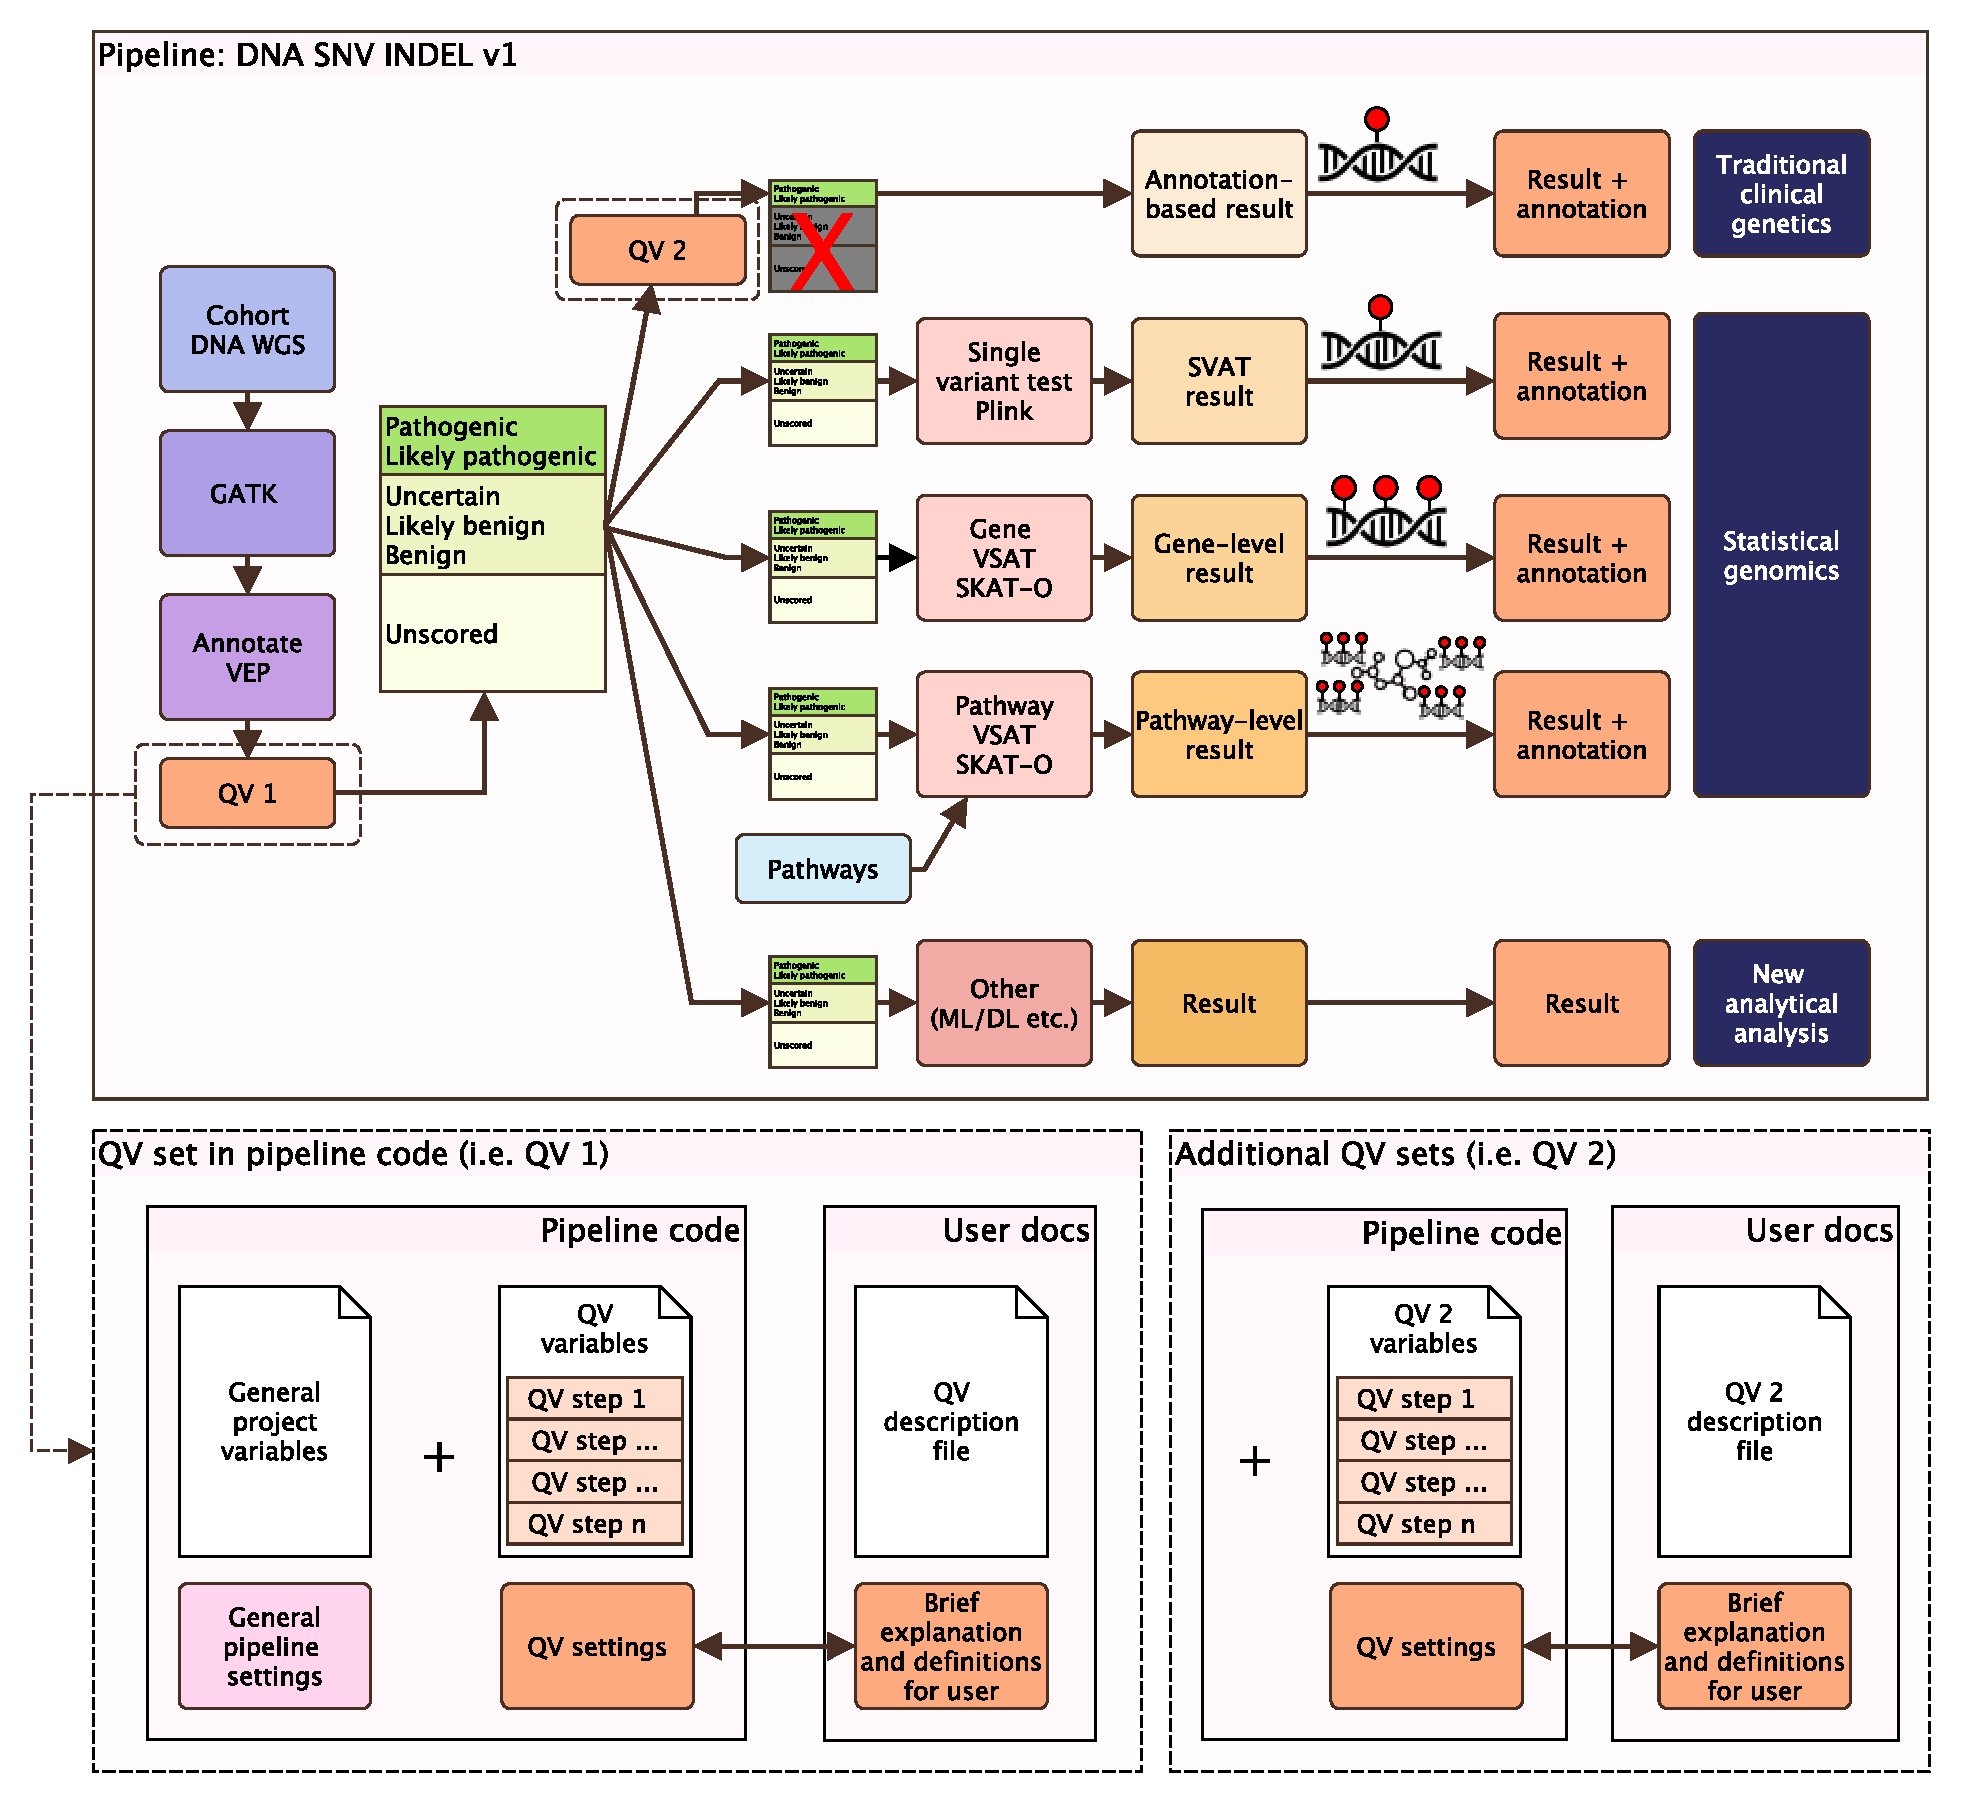
\includegraphics[width=0.99\textwidth]{./images/qv_pipeline_with_file_vcurrent.pdf}
    \caption{Summary of the example application design for the DNA SNV INDEL v1 pipeline. \ac{qv}1 and \ac{qv}2 are shown as sequential and potentially piped protocol steps. The description file (non-mandatory) and the variables file (mandatory) form part of the QV files that are loaded by the analysis pipeline. This illustration highlights a single stage in the QV1 set (i.e. step 10 where the GATK VQSR method is applied), with the full pipeline simplified under the QV1 icon.}
    \label{fig:qv_pipeline_with_file_vcurrent}
\end{figure}

The typical representation of \ac{qv} steps is shown in \textbf{figure \ref{fig:qv_filter_pyramid_vcurrent}}.
This figure summarises the common steps in the variant filtering process such as \ac{qc} filtering of raw omic data,
removing background noise such as high frequency variants compared to a reference population, and filtering on variant effect metrics like pathogenicity scores.
The transition from raw data to annotated variants, as illustrated in \textbf{figure \ref{fig:candidate_variants_sequence_annotation}}, underscores how initial \ac{qv} steps (e.g. \ac{qc}) are complemented by additional filtering based on new annotation data.
 
\begin{SCfigure}[][h]
%\begin{figure}[h]
\centering
     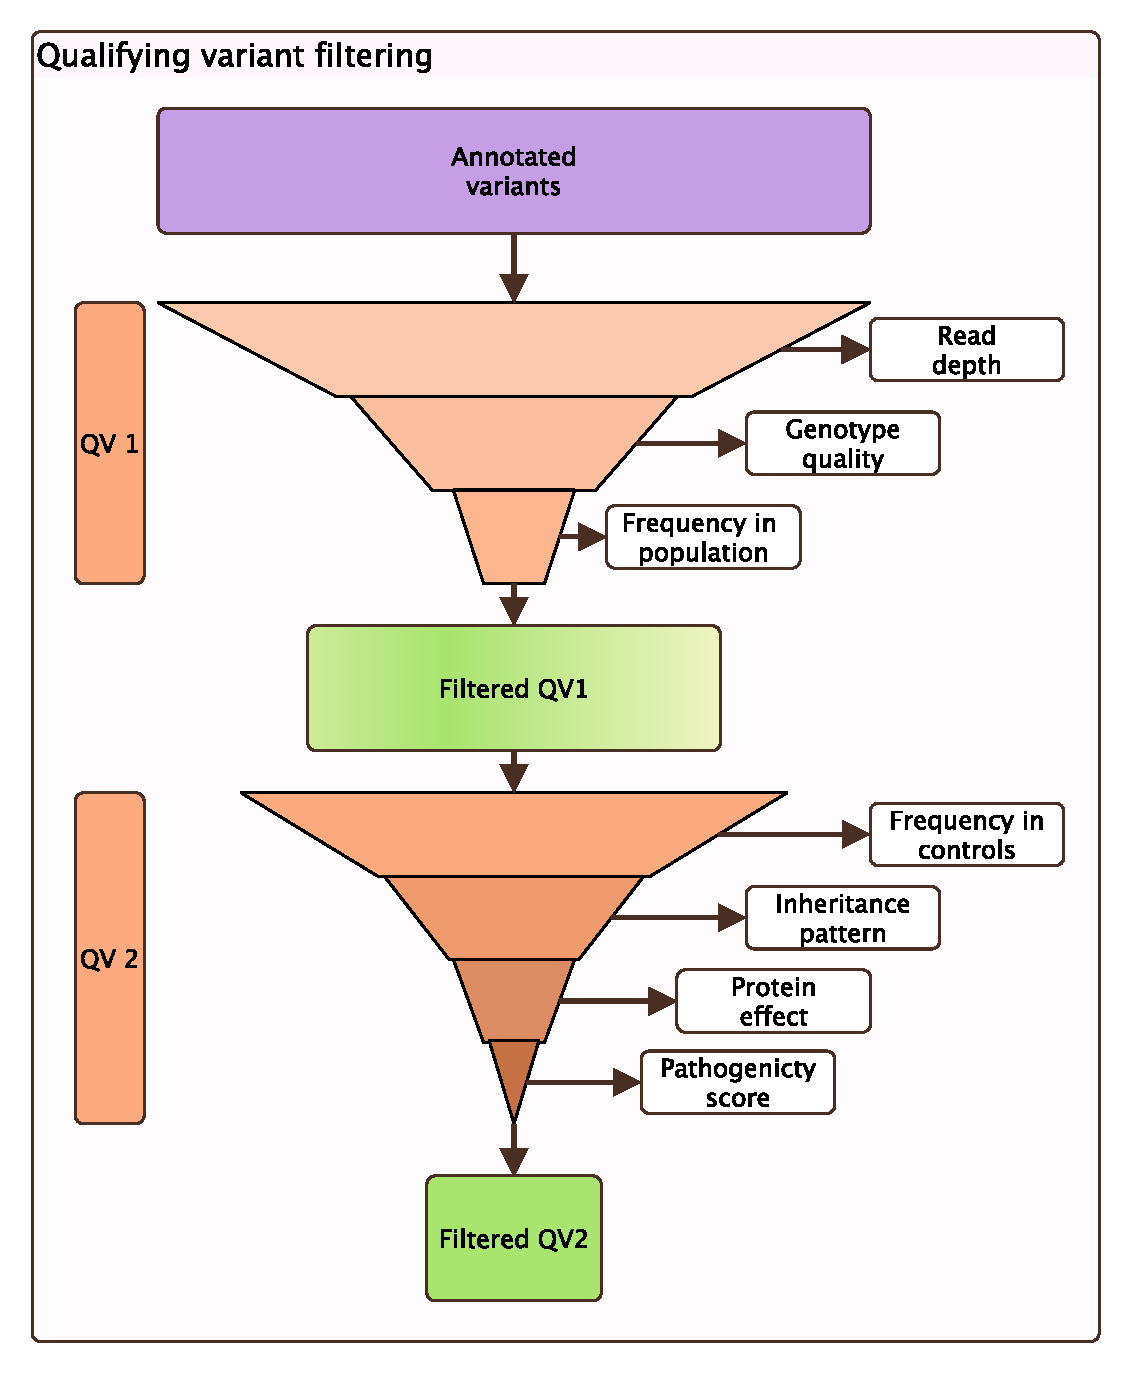
\includegraphics[width=0.66\textwidth]{./images/qv_filter_pyramid_vcurrent.pdf}
\caption{Illustration of the qualifying variant workflow. Each layer of filtering can arise from different stages of the pipeline. In reality, we observe that each layer of the filters comes from disparate stages of a pipeline.}
    \label{fig:qv_filter_pyramid_vcurrent}
% \end{figure}
\end{SCfigure}

Previous work has demonstrated tangible applications of \ac{qv}s. For instance, \citet{povysil2019rare} provided an example of \ac{qv}s in variant collapsing analyses for complex traits, while \citet{cirulli2015exome} introduced the concept in early studies. Despite these contributions, a standardised framework for presenting \ac{qv}s is absent. Here, we detail four typical applications of \ac{qv} sets:
\begin{enumerate}
    \item \textbf{\ac{qv} passing \ac{qc} only}: Generates large datasets (e.g. 500,000 variants per subject) for \ac{gwas} or initial \ac{wgs} pre-processing.
    \item \textbf{Flexible \ac{qv}}: Balances between \ac{qc} and false positives, yielding intermediate datasets (e.g. fewer than 100,000 variants per subject) for rare variant association testing.
    \item \textbf{\ac{qv} for rare disease}: Applies stringent filtering to produce smaller datasets (e.g. around 1,000 variants per subject), targeting known genes or single causal variants.
    \item \textbf{Known disease panel \ac{qv} set}: Utilises well-established gene panels with pathogenic variants (e.g. the \ac{acmg} \ac{sf} set) for clinical reporting \cite{miller2023acmg}.
\end{enumerate}

Two exemplary applications of \ac{qv}s are found in clinical genetics reporting and \ac{gwas}. In clinical genetics, single-case analyses may select \ac{qv}s from disease-causing gene lists provided by expert panels, with variants being categorised as \ac{vus}, known, candidate, or causal. In \ac{gwas}, \ac{qv}s typically represent consensus variants that have passed rigorous \ac{qc} procedures, ensuring their suitability for statistical analyses. The careful selection and categorisation of \ac{qv}s are thus critical for accurate reporting and reproducibility, sometimes even more so than the choice of the analysis pipeline itself \cite{olson2023variant}.

\begin{figure}[h!]
    \centering
   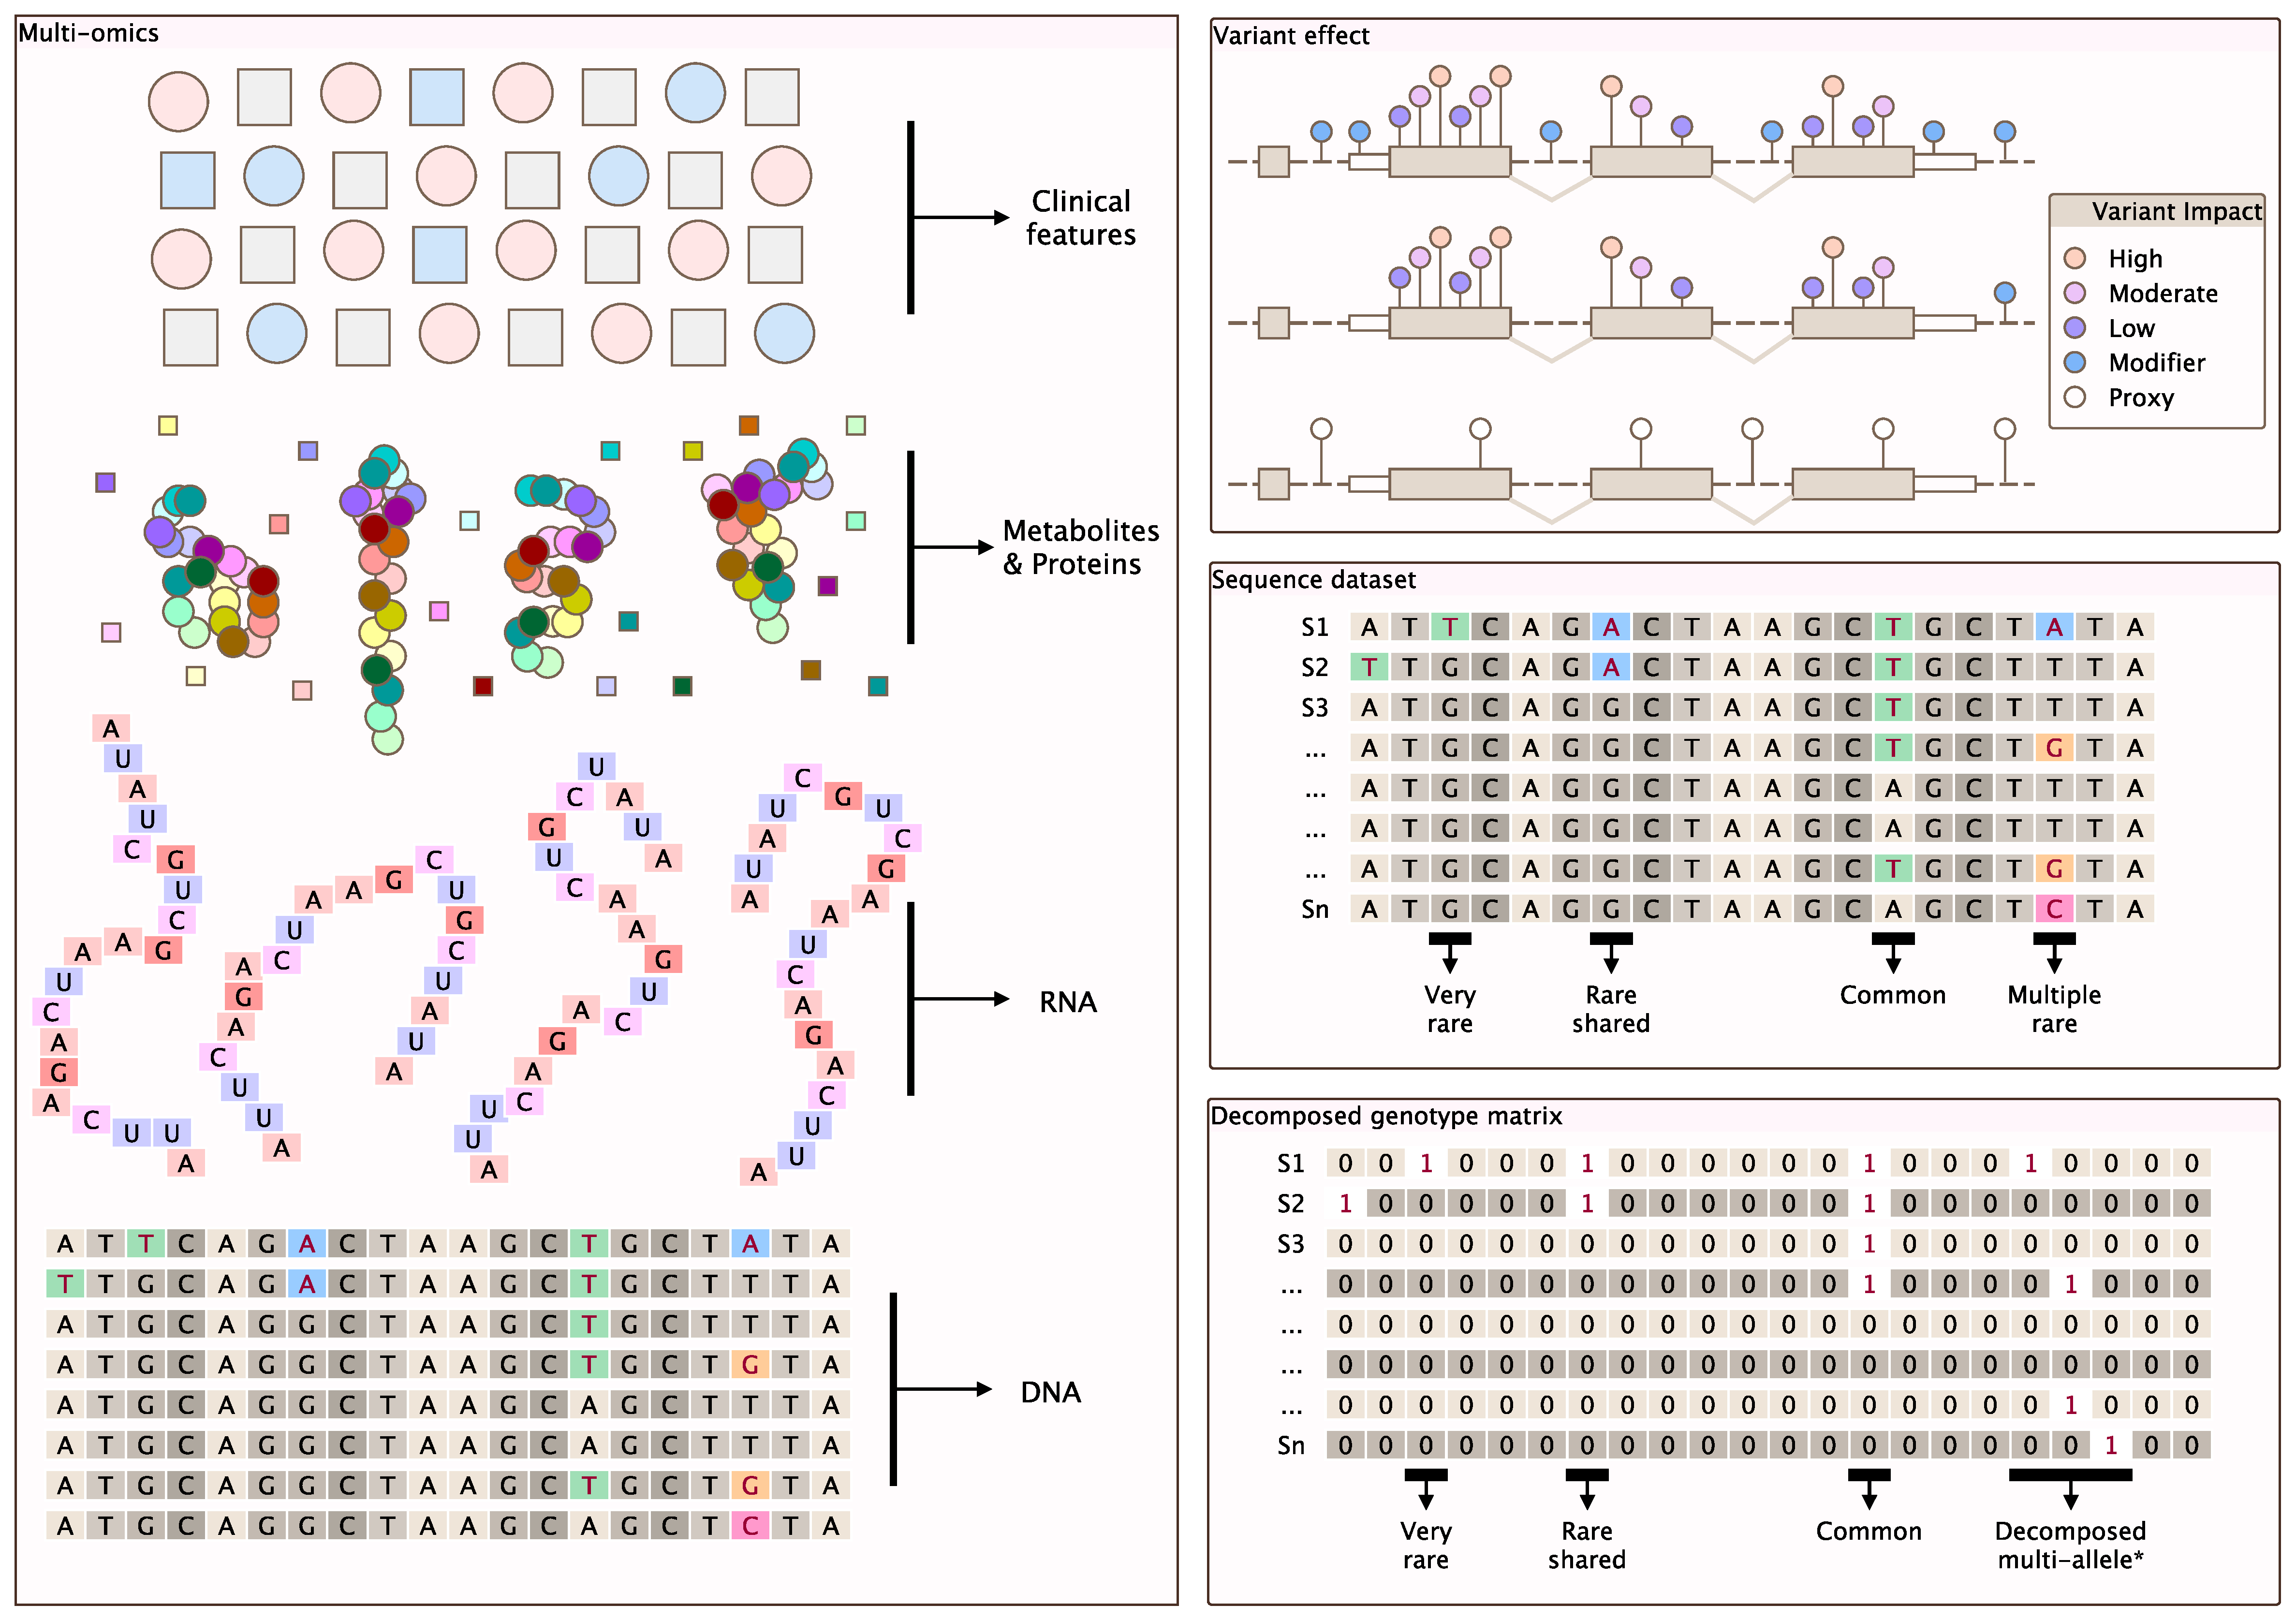
\includegraphics[width=0.8\textwidth]{./images/candidate_variants_sequence_to_matrix_pink.pdf}
      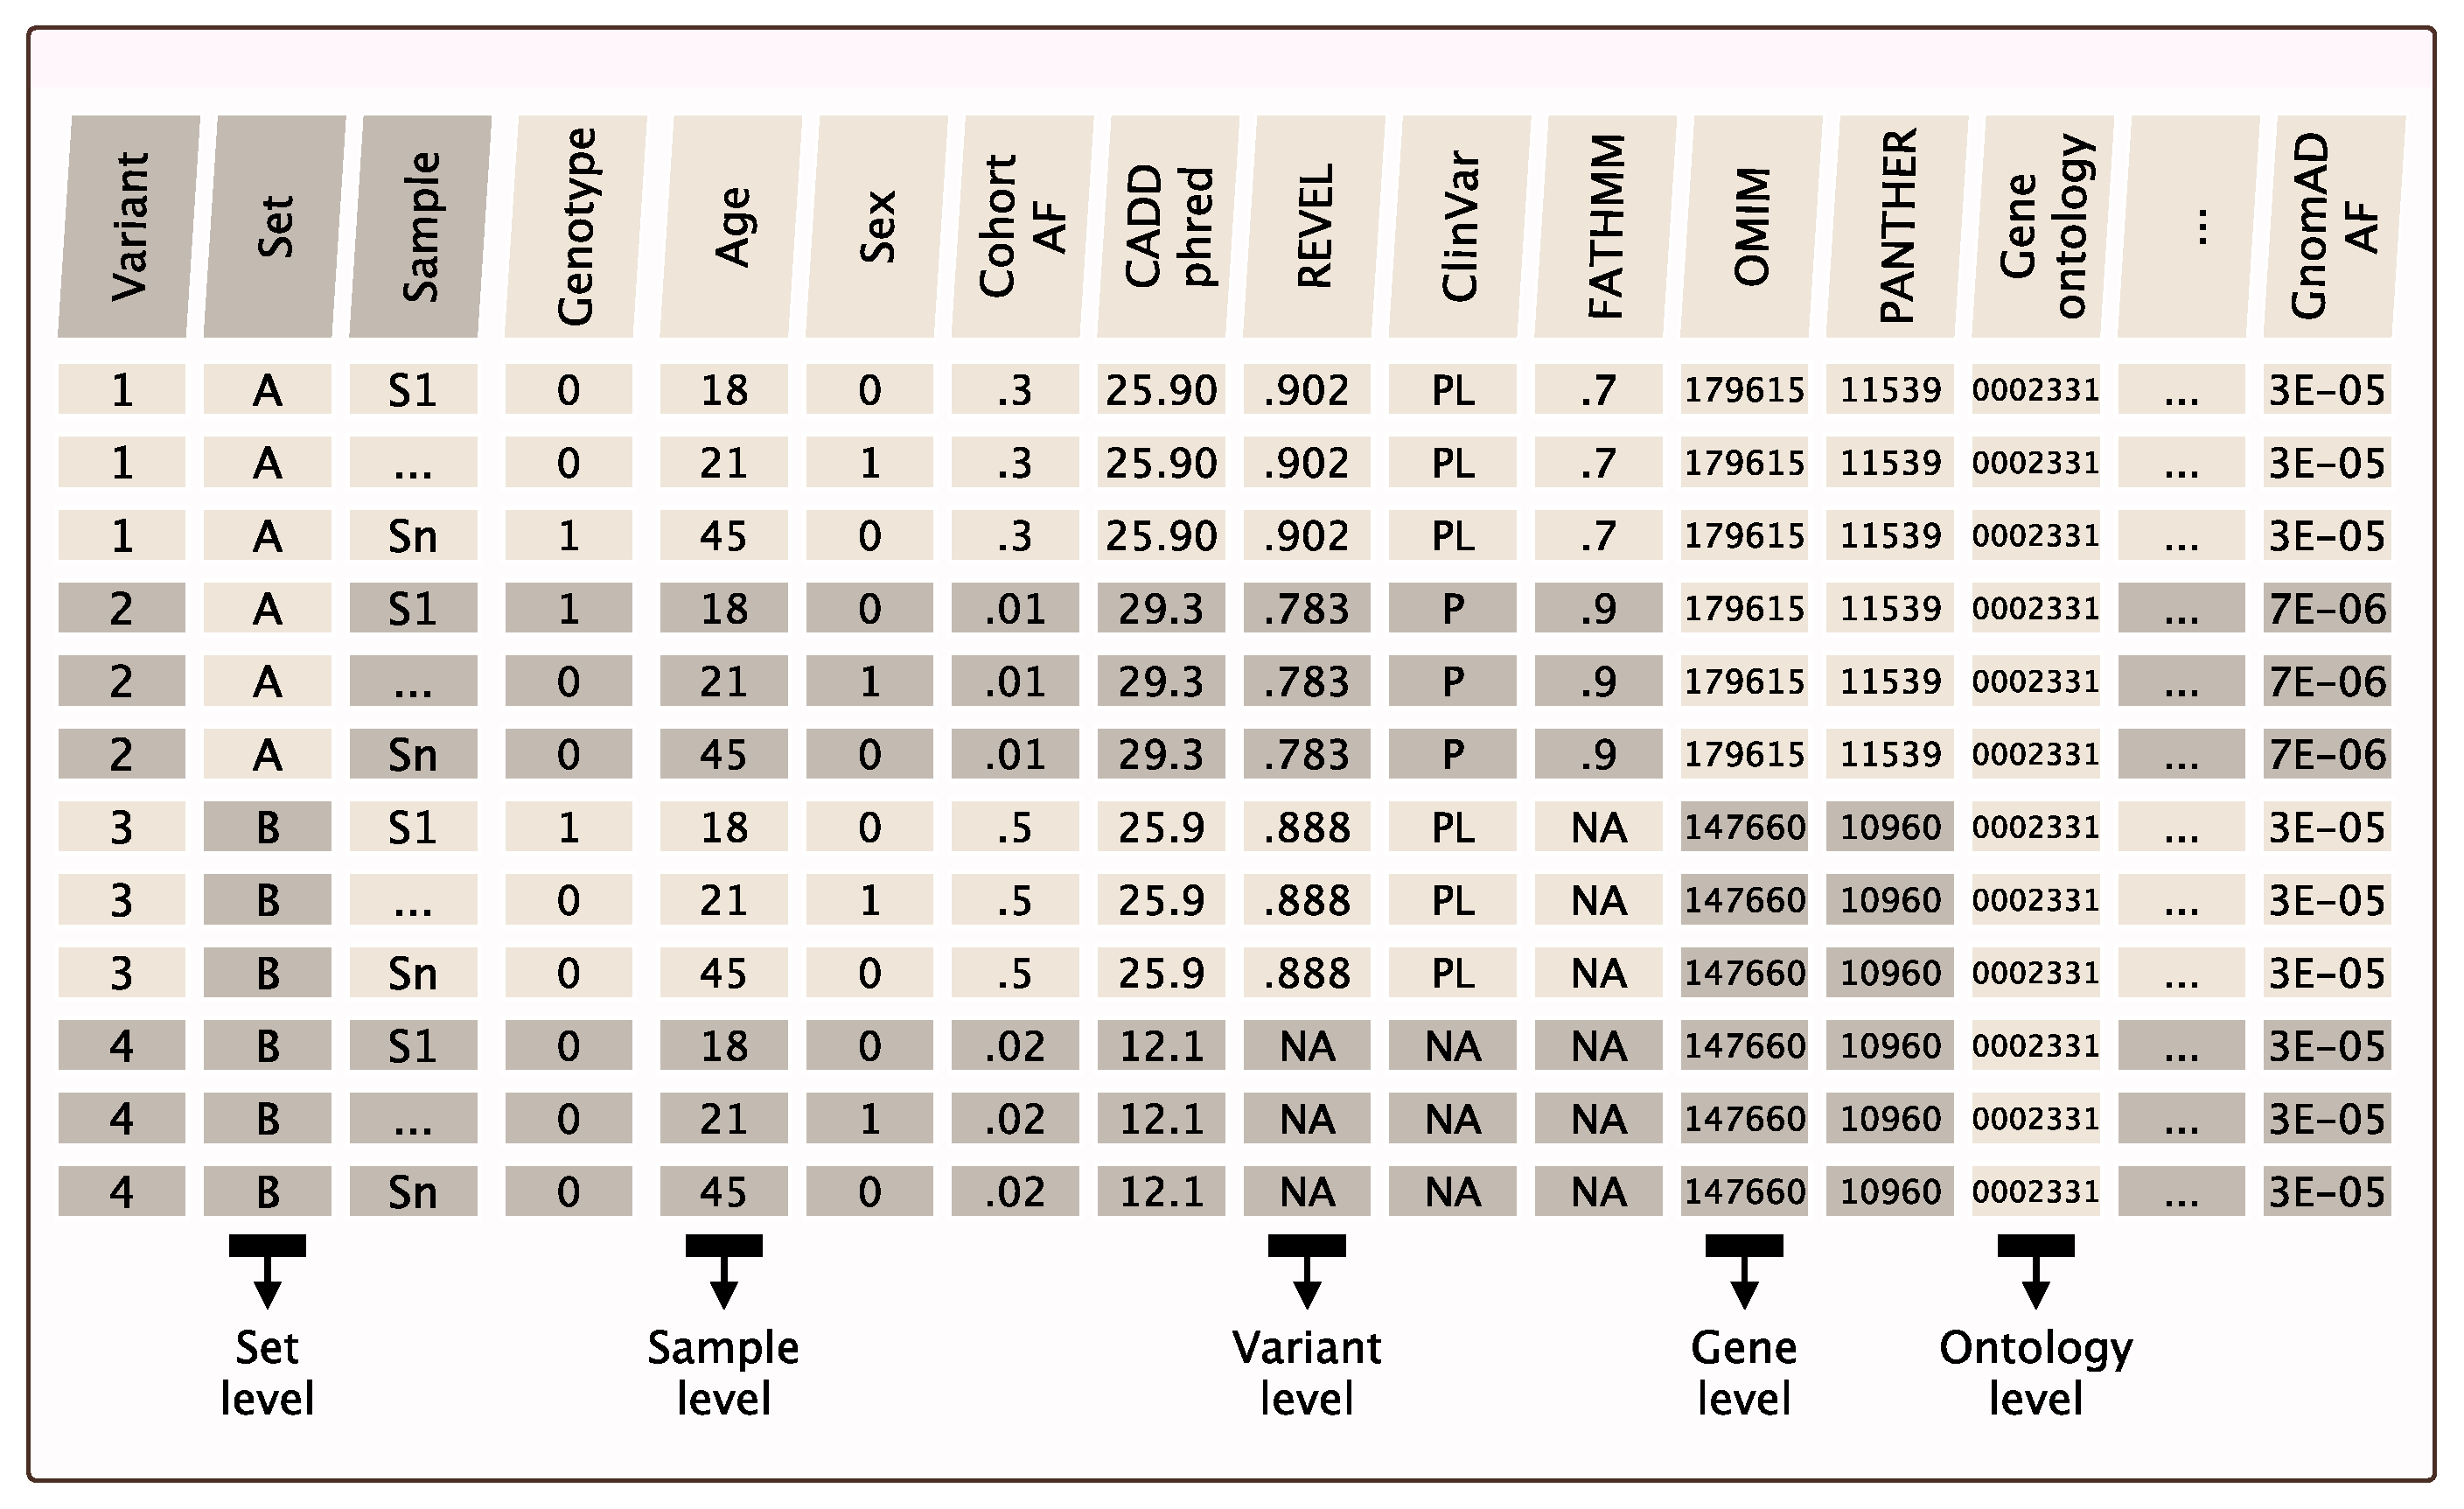
\includegraphics[width=0.8\textwidth]{./images/candidate_variants_sequence_annotation_pink.pdf}
    \caption{
Top: Transformation from raw omic data to a data matrix. Bottom: Initial variant detection requires \ac{qc} and filtering rules, which are the first \ac{qv} steps. Subsequent annotation of variants enables further \ac{qv} filtering based on new information.    
    }
        \label{fig:candidate_variants_sequence_annotation}
\end{figure}

\subsection{Background problem and proposed solution}

As study sizes now exceed one million subjects \cite{lee2018gene, jansen2019genome}, the shift from genotyping to \ac{wgs} is now standard, allowing rare variants to be included in \ac{gwas} and \ac{vsat} for more comprehensive analyses of complex traits \cite{manolio2009finding, young2019solving}. % These paper describes the concept of ‘missing heritability’, the observation that heritability estimates from \ac{gwas} are much lower than those from twin studies.
\ac{qv} protocols play a crucial role in data cleaning and preparation, ensuring the integrity of subsequent analyses. Although the term ``\ac{qv}'' is often used as a catch-all descriptor for various filtering steps, in practice it encompasses multiple stages that originate from diverse parts of the pipeline.
\textbf{Figure \ref{fig:qv_structure_vcurrent}} illustrates the structural framework of an annotated variant, highlighting the features, both pre-existing metadata and post-calling annotations, that can trigger specific \ac{qv} protocols. This figure emphasises that each variant is subject to multiple criteria, which may derive from distinct processing steps.

\begin{figure}[h!]
\centering
     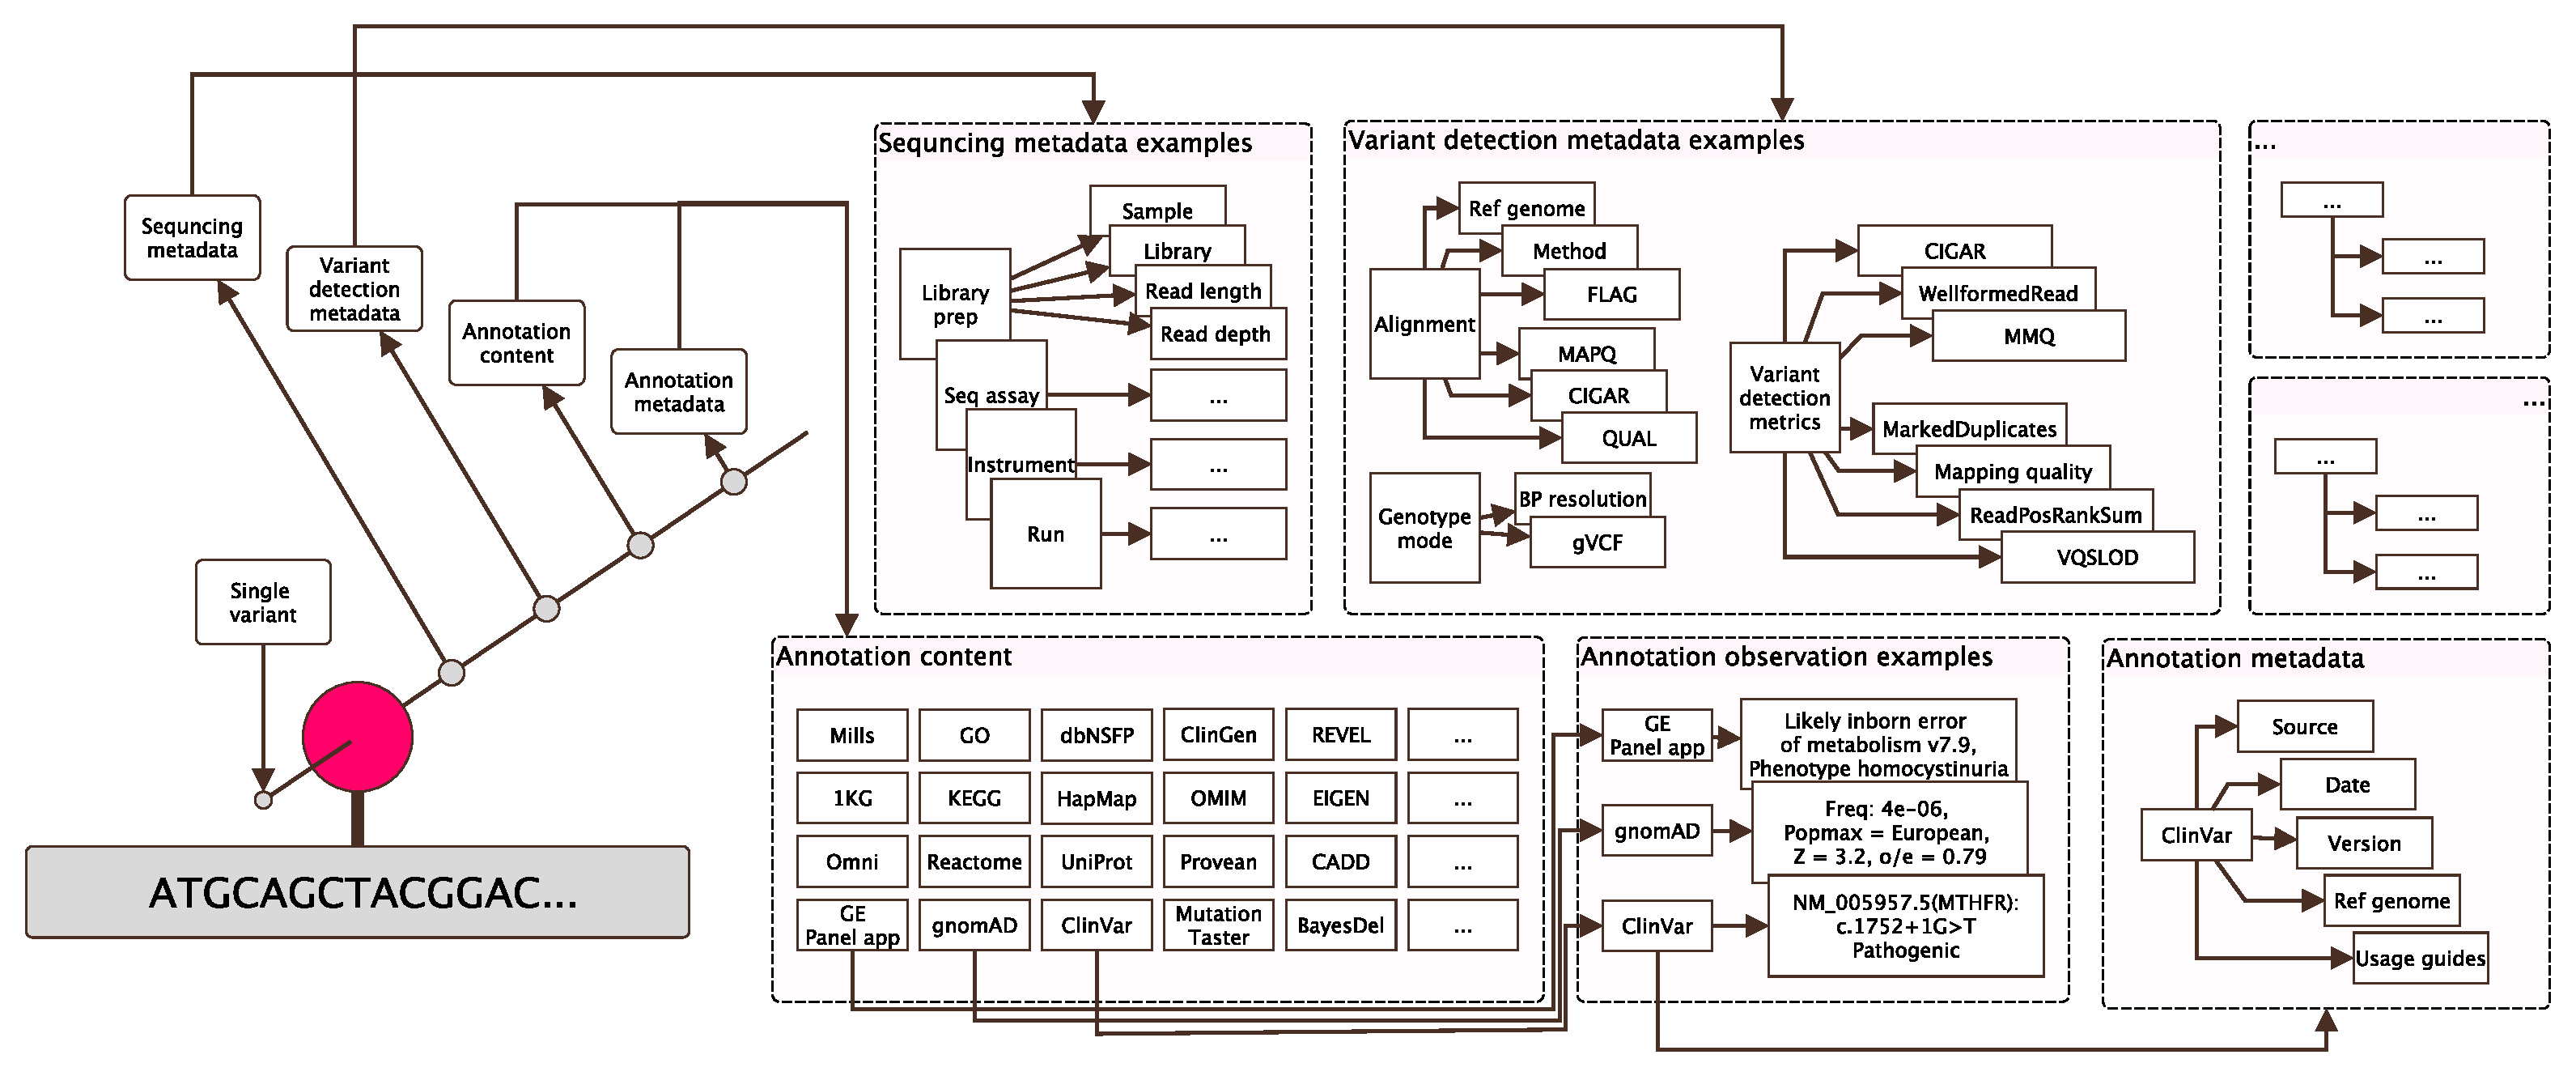
\includegraphics[width=0.99\textwidth]{./images/qv_structure_vcurrent.pdf}
\caption{
Structural framework of an annotated variant. The diagram highlights selected features, both pre-existing metadata and annotations added after variant calling, that can trigger specific \ac{qv} protocols.
}
\label{fig:qv_structure_vcurrent}
\end{figure}

Moreover, complex analyses often require multiple processing streams that are ultimately merged into a cohesive result. A standardised \ac{qv} format would allow for the use of various \ac{qv} sets, each based on different filters and variables, while providing a common foundation for consistency across disparate data streams. The ambiguity in the term \ac{qv} across genomic studies underscores the need for a clear and flexible definition that captures both its common uses and its implementation across multiple stages.

By introducing a new vocabulary and a standard reference model for \ac{qv}s, we aim to clarify the concept and improve communication and methodological discussion across disciplines for more advanced tasks.
We define and exemplify several common \ac{qv} sets, illustrating their potential configurations and roles within analysis pipelines:
\begin{enumerate}
    \item Theoretical pipelining of \ac{qv} sets.
    \item Establishment of standardised \ac{qv} sets for specific analytical scenarios.
    \item Recognition that \ac{qv}s are integral throughout the analysis pipeline rather than confined to a single end-stage.
\end{enumerate}

The proposed QV framework provides structured, human- and machine-readable definitions to standardise the selection and interpretation of variants across diverse genomic studies. This methodology promotes efficient and precise variant detection and interpretation, essential for both research and clinical diagnostics. 
Moreover, the structured criteria adhere to the principles of \ac{fair} \cite{wilkinson2016fair}. 
In \textbf{section \ref{semantic}} we discuss how they can be versioned and integrated using standard vocabularies (e.g. SNOMED CT, \ac{sphn} \ac{rfd} Schema), assigned unique identifiers (via SHA-256 hashes, UUIDs, or semantic combinations), and provided in human- and machine-readable formats such as YAML and \ac{rdf}, ensuring seamless integration across databases and platforms.

\section{Results}

In the following sections, we first present a high-level view of a complete analysis using our \ac{qv} framework 
(\textbf{sec \ref{sec:example_high_level}}), illustrating its application in diverse contexts such as a multi-part genomic analysis. We then introduce the underlying methodological framework 
(\textbf{sec \ref{sec:framework}}), followed by an explicit example of one individual step (\textbf{ sec \ref{sec:protocol_variables_example}}) to demonstrate how \ac{qv} criteria are integrated into a pipeline. This specific example use the \ac{vqsr} step from the 
\ac{gatk} \ac{wgs} workflow \cite{auwera_genomics_2020} - a typical pipeline step.

\subsection{Application of Qualifying Variants and an Example Use Case}\label{sec:example_high_level}

We examine scenarios where \ac{qv}s have proved essential, including applications in \ac{gwas}, \ac{wgs} and clinical genetics. In large-scale studies and rare disease research, for example, sophisticated risk models that integrate clinical and genomic data can significantly enhance predictive accuracy in well-defined cohorts \cite{riveros2021integrated, weale2021validation, sun2021polygenic}. Similarly, standardised \ac{qv} protocols support reproducibility across studies, particularly when analysing complex signals in isolated populations \cite{lim2014distribution}.

%\subsubsection{Example application of qualifying variants in WGS analysis}
Multiple \ac{qv} protocols can be combined to generate progressively filtered datasets tailored to specific analytical needs. Often, different \ac{qv} sets are applied sequentially, with the final outcomes merged to address distinct objectives. For instance, a comprehensive analysis pipeline might integrate:
\begin{itemize}
  \item \colorbox{kispiblue!30}{\texttt{QV SNV/INDEL}},
  \item \colorbox{kispiblue!30}{\texttt{QV CNV}},
  \item \colorbox{kispiblue!30}{\texttt{QV structural variation}},
  \item \colorbox{kispiblue!30}{\texttt{QV rare disease known}}, and 
  \item \colorbox{kispiblue!30}{\texttt{QV statistical association \ac{qc}}}.
\end{itemize}
The final analysis yields (1) a joint cohort disease association (e.g. variant P-values) and (2) individual single-case results (e.g. clinical genetics diagnosis for a patient)
\cite{auwera_genomics_2020, li2025statistical}.

As an example, we focus on a SNV/INDEL pipeline employing two \ac{qv} sets:
\colorbox{colorSUNSET2!60}{\texttt{QV SNV INDEL v1}} for flexible cohort-level filtering, and 
\colorbox{colorSUNSET2!60}{\texttt{QV SNV INDEL v2}} for stricter filtering in subsequent single-case analysis. The pipeline is illustrated in \textbf{Box \ref{box:pipe}}, and can be summarised as follows:

\begin{quotation}
A cohort of patient WGS data was analysed to identify genetic determinants for phenotype X. Initially, a flexible \ac{qv} set (\texttt{QV SNV INDEL v1}) was applied using the 
\colorbox{colorSUNSET1!30}{\texttt{pipeline DNA SNV INDEL v1}}, which implements the \texttt{QV SNV INDEL v1} criteria to produce the prepared dataset (\colorbox{colorSUNSET3!30}{\texttt{dataset DNA SNV INDEL v1}}). This dataset was then analysed alongside other modules (e.g. \colorbox{colorSUNSET4!30}{\texttt{PCA SNV INDEL v1}} and \colorbox{colorSUNSET5!30}{\texttt{statistical genomics v1}}) to derive a cohort-level association signal (Result 1). Next, the same prepared dataset was re-filtered with the stricter \texttt{QV SNV INDEL v2} criteria to identify known causal variants for each patient, yielding the final dataset (\colorbox{colorSUNSET3!30}{\texttt{dataset DNA SNV INDEL v2}}) and resulting in individual case reports (Result 2).
\end{quotation}

\begin{tcolorbox}[
    colback=white!0,
    colframe=black,
    boxrule=1pt,
    arc=1mm,
    outer arc=1mm,
    title=\textbf{\refstepcounter{myboxcounter}\label{box:pipe}Box \themyboxcounter: Example diagrammatic representation}
]
\dirtree{%
.1 \colorbox{colorSUNSET1!30}{\texttt{pipeline DNA SNV INDEL v1}}.
.2 Flexible \ac{qv} criteria.
.3 \colorbox{colorSUNSET2!60}{\texttt{QV SNV INDEL v1}} $\rightarrow$ \colorbox{colorSUNSET3!30}{\texttt{dataset DNA SNV INDEL v1}}.
.4 \colorbox{colorSUNSET4!30}{\texttt{PCA SNV INDEL v1}}.
.4 \colorbox{colorSUNSET5!30}{\texttt{statistical genomics v1}} $\rightarrow$ Result 1.
.3 \colorbox{colorSUNSET3!30}{\texttt{dataset DNA SNV INDEL v1}}.
.4 Rare disease \ac{qv} criteria.
.5 \colorbox{colorSUNSET2!60}{\texttt{QV SNV INDEL v2}} $\rightarrow$ \colorbox{colorSUNSET3!30}{\texttt{dataset DNA SNV INDEL v2}}.
.6 \colorbox{colorSUNSET5!30}{\texttt{single case report SNV INDEL v1}} $\rightarrow$ Result 2.
.3 Joint analysis output.
}
\medskip

Joint analysis output from:\\
Result 1 = Cohort-level association signal (e.g. variant P-value).\\
Result 2 = Single variant report per patient.
\end{tcolorbox}


\subsection{Methodological framework} \label{sec:framework}
We introduce a simple framework for the effective use of \ac{qv}  protocols. This framework comprises three components, as illustrated in \textbf{Figure \ref{fig:qv_pipeline_with_file_vcurrent}}:
\begin{enumerate}
    \item \textbf{Variables}: The criteria variables that are sourced as part of the pipeline (see \textbf{Box \ref{box:qv_variables_example}}).
    \item \textbf{Description}: A narrative of each step within the overall QV set (see \textbf{Box \ref{box:qv_description_example}}).
    \item \textbf{Source code}: The implementation of the variables file within the pipeline code (see \textbf{Box \ref{box:qv_bash_code_example}}).
\end{enumerate}

This framework efficiently manages \ac{qv}-specific variables (e.g. allele frequency thresholds) separately from general pipeline settings, thereby maintaining clarity and specificity. We first present a detailed example using \ac{vqsr} from the \ac{qv} set \colorbox{colorSUNSET2!60}{\texttt{QV SNV INDEL v1}} to illustrate the practical application of this method in a real-world genomic analysis scenario. We later demonstrate how this approach integrates with workflow managers such as Snakemake \cite{molder_sustainable_2021} or Nextflow \cite{di_tommaso_nextflow_2017}, streamlining genomic processing tasks.

Individual steps within \ac{qv} criteria may be categorised into different types. For organisational purposes, we recommend using simple labels such as ``\ac{qc}'' and ``filter''. For example: (1) Filtering thresholds (e.g. \ac{af} $>$ 0.1 in a cohort, $<$ 0.1 in gnomAD) may be directly applied to exclude affected variants. (2) Multiple steps involving annotation-based criteria (e.g. \ac{qc} flags) may not remove variants immediately but enable downstream analyses that depend on several \ac{qv} criteria.
In a QC protocol, one step might filter variants based solely on threshold values (criteria 1), while another may combine several upstream QC criteria (criteria 2).

\subsubsection{Detailed example of QV variables}\label{sec:protocol_variables_example}
As a detailed example, we focus on the \colorbox{kispiblue!30}{\texttt{vqsr}} step from the \ac{qv} set \colorbox{colorSUNSET2!60}{\texttt{QV SNV INDEL v1}}. The process is illustrated in three parts.
First, the mandatory QV variables are set (see \textbf{Box \ref{box:qv_variables_example}}).
Second, an optional description is provided (see \textbf{Box \ref{box:qv_description_example}}).
Third, the variables are integrated into the source code (see \textbf{Box \ref{box:qv_bash_code_example}}).

\begin{tcolorbox}[
    breakable,  % Allows the box to split over pages
    colback=white!0,  % No background color (fully transparent)
    colframe=black,  % Black border color
    boxrule=1pt,  % Width of the border
    arc=1mm,  % Radius of the corner rounding
    outer arc=1mm,
%    title=\textbf{1. Example QV variables - extract from QV1 variables file}
     title=\textbf{\refstepcounter{myboxcounter}\label{box:qv_variables_example}Box \themyboxcounter: Example QV variables - extract from QV1 variables file}
]

\begin{verbatim}
# VQSR SNP Mode Variables
vqsr_snp_hapmap_known="false"
vqsr_snp_hapmap_training="true"
vqsr_snp_hapmap_truth="true"
vqsr_snp_hapmap_prior="15.0"

vqsr_snp_omni_known="false"
vqsr_snp_omni_training="true"
vqsr_snp_omni_truth="false"
vqsr_snp_omni_prior="12.0"

vqsr_snp_1000g_known="false"
vqsr_snp_1000g_training="true"
vqsr_snp_1000g_truth="false"
vqsr_snp_1000g_prior="10.0"

vqsr_snp_annotations="QD,MQ,MQRankSum,ReadPosRankSum,FS,SOR"
vqsr_snp_truth_sensitivity="99.7"
\end{verbatim}
\end{tcolorbox}

\begin{tcolorbox}[
    breakable,  % Allows the box to split over pages
    colback=white!0,  % No background color (fully transparent)
    colframe=black,  % Black border color
    boxrule=1pt,  % Width of the border
    arc=1mm,  % Radius of the corner rounding
    outer arc=1mm,
%    title=\textbf{2. }
         title=\textbf{\refstepcounter{myboxcounter}\label{box:qv_description_example}Box \themyboxcounter: Example QV descriptions - extract from QV1 variables file}
]


\begin{enumerate}
    \item \textbf{[\ac{qc}]} \colorbox{kispiblue!30}{\texttt{fastp}}: Performs initial read quality ...
    \item \textbf{[\ac{qc}]} \colorbox{kispiblue!30}{\texttt{collectwgsmetrics}}: Assesses BAM file ...
    \item \textbf{[\ac{qc}]} \colorbox{kispiblue!30}{\texttt{rmdup\_merge}}: Marks duplicate reads ...
    \item \textbf{[\ac{qc}]} \colorbox{kispiblue!30}{\texttt{haplotype\_caller}}: Generates gVCF using \texttt{-ERC GVCF} ...
    \item \textbf{[\ac{qc}]} \colorbox{kispiblue!30}{\texttt{vqsr}}: Performs Variant Quality Score Recalibration (VQSR) using GATK. In this step, SNP mode is applied with three reference resources: \textbf{HapMap} is used as a high-confidence reference (training=true, truth=true, prior=15.0), \textbf{Omni} provides supplementary training data (training=true, truth=false, prior=12.0), and \textbf{1000G} informs on common SNP variation (training=true, truth=false, prior=10.0). Additionally, VQSR uses key annotations (QD, MQ, MQRankSum, ReadPosRankSum, FS, SOR) and applies a truth sensitivity filter of 99.7\% to retain high-confidence variants.
   \item \textbf{[\ac{qc}]} ...
\end{enumerate}


\end{tcolorbox}

\begin{tcolorbox}[
    breakable,  % Allows the box to split over pages
    colback=white!0,  % No background color (fully transparent)
    colframe=black,  % Black border color
    boxrule=1pt,  % Width of the border
    arc=1mm,  % Radius of the corner rounding
    outer arc=1mm,
%    title=\textbf{3. Example code sourcing the variables file}
    title=\textbf{\refstepcounter{myboxcounter}\label{box:qv_bash_code_example}Box \themyboxcounter: Example code sourcing the variables file}
]

\lstinputlisting{example_qv_code.sh}
\end{tcolorbox}

\subsubsection{Simple example with a workflow manager}
We demonstrate the use of a \ac{qv} variable file within a workflow manager, such as Snakemake or Nextflow
(\textbf{box \ref{box:qv_variables_example_workflow1}}).
The setup involves two types of YAML configuration files: one for general pipeline settings and another specifically for \ac{qv}-related variables
(\textbf{box \ref{box:qv_variables_example_workflow2}}).
These configurations are integrated into the primary analysis script, typically a Snakefile, ensuring that all parameters required for genomic analyses are systematically managed and applied 
(\textbf{box \ref{box:qv_variables_example_workflow3}}). 

\begin{tcolorbox}[
    breakable,  % Allows the box to split over pages
    colback=white!0,  % No background color (fully transparent)
    colframe=black,  % Black border color
    boxrule=1pt,  % Width of the border
    arc=1mm,  % Radius of the corner rounding
    outer arc=1mm,
%    title=\textbf{1. Example QV variables - extract from QV1 variables file}
     title=\textbf{\refstepcounter{myboxcounter}\label{box:qv_variables_example_workflow1}Box \themyboxcounter: Example worflow manager - yaml}
]

\begin{verbatim}
# qv_config.yaml
min_depth: 10
max_allele_frequency: 0.01
quality_score_threshold: 20
\end{verbatim}
\end{tcolorbox}

\begin{tcolorbox}[
    breakable,  % Allows the box to split over pages
    colback=white!0,  % No background color (fully transparent)
    colframe=black,  % Black border color
    boxrule=1pt,  % Width of the border
    arc=1mm,  % Radius of the corner rounding
    outer arc=1mm,
%    title=\textbf{1. Example QV variables - extract from QV1 variables file}
     title=\textbf{\refstepcounter{myboxcounter}\label{box:qv_variables_example_workflow2}Box \themyboxcounter: Example worflow manager - yaml}
]
\begin{verbatim}
# config.yaml
reference_genome: "path/to/reference/genome.fasta"
annotation_file: "path/to/annotation.gtf"
sample_list: "path/to/samples.txt"
output_dir: "path/to/output"
qv_config: "qv_config.yaml"
\end{verbatim}
\end{tcolorbox}



\begin{tcolorbox}[
    breakable,  % Allows the box to split over pages
    colback=white!0,  % No background color (fully transparent)
    colframe=black,  % Black border color
    boxrule=1pt,  % Width of the border
    arc=1mm,  % Radius of the corner rounding
    outer arc=1mm,
%    title=\textbf{1. Example QV variables - extract from QV1 variables file}
     title=\textbf{\refstepcounter{myboxcounter}\label{box:qv_variables_example_workflow3}Box \themyboxcounter: Example worflow manager - python}
]
\begin{verbatim}
# Snakefile
configfile: "config.yaml"
qv_settings = read_yaml(config["qv_config"])

rule all:
  input:
    "results/filtered_variants.vcf"

rule filter_variants:
  input:
    "data/raw_variants.vcf"
  output:
    "results/filtered_variants.vcf"
  params:
    depth = qv_settings['min_depth'],
    af = qv_settings['max_allele_frequency'],
    qs = qv_settings['quality_score_threshold']
  shell:
    """
    bcftools filter -i 'DP>{depth} && AF<{af} && \
    QUAL>{qs}' {input} > {output}
    ""
\end{verbatim}
\end{tcolorbox}

\subsection{Examples of real-world QV applications}

\subsubsection{Discovery research}
\citet{greene2023genetic} provide an example of \ac{qv} standardisation with their ``Rareservoir'', a relational database schema optimised for rare disease studies. This database focuses on rare variants (those with a \ac{maf} below 0.1\%), reducing data size by approximately 99\% by storing variants as 64-bit integers (``RSVR IDs'') and organising them by genomic position for efficient querying. Additional data, such as \ac{maf}s from gnomAD, CADD pathogenicity scores and impact predictions per the Sequence Ontology, are encoded into a 64-bit integer (``CSQ ID''), where each bit corresponds to a specific gene function impact, ranked by severity. By employing the Bayesian genetic association method BeviMed, initially described by \citet{greene2017fast}, the study effectively inferred associations between genes and rare disease phenotypes, demonstrating the capacity to handle and analyse complex genetic datasets. The protocol of \citet{greene2023genetic} can be reproduced in the \ac{qv} format, thereby facilitating interpretation and reproducibility.

In our work, we are applying the \ac{qv} framework within ``SwissPedHealth'', a national paediatric data stream aimed at investigating rare or unknown diseases using a multiomic approach including \ac{wgs}, RNAseq, proteomics, metabolomics, and clinical data \cite{mozun2024paediatric}. The SwissPedHealth Lighthouse project involves approximately 450 paediatric cases with rare, life-threatening conditions, with the goal of improving diagnosis by integrating clinical data with multiomics. By using consensus raw datasets (e.g. WGS in patients and families) that are annotated and filtered to multiple \ac{qv} levels, we generate pre-processed datasets suitable for a range of analyses, including \ac{gwas}, \ac{vsat}, single-case clinical genetics reporting, machine learning, and joint multiomic studies.

This approach aligns with practices in large-scale national projects, such as the Genomics England 100,000 Genomes Project, which performs central automated analysis with interpretation and clinical reporting \cite{turnbull2018100}. Although such projects currently embed \ac{qv} protocols throughout their pipelines without explicit standardisation, our method aims to improve consistency and reproducibility. Moreover, the increasing importance of \ac{qv} protocols in genomics-based newborn screening, a rapidly emerging healthcare innovation \cite{noauthor_every_2024}, highlights the critical role of standardised variant filtering in bridging research and clinical practice.

\subsubsection{Rapid diagnostics}
% WGS diagnostic
Screening for known diseases typically involves searching for a predefined \ac{qv} set. The adoption of a formalised standard would enhance consistency and reliability for stakeholders. For instance, genome analysis in neurodevelopmental disorders in 465 families identified causal variants in 36\% of 489 affected individuals \citep{sanchis2023genome}, while the DDD study, involving over 13,500 families, achieved a genetic diagnosis in approximately 41\% of probands \cite{wright2023genomic}. In addition, genomic lifespan association studies in Iceland, which included 57,933 participants, identified 2,306 individuals with actionable genotypes associated with a reduction in median lifespan by around three years \citep{jensson2023actionable}.

% speed
Rapid genomic diagnostics can be further enhanced by the use of standardised \ac{qv} protocols. Standardisation of \ac{qv} filtering ensures high-confidence in the analysis protocol, thereby streamlining data interpretation, reproducibility, and meta analysis. For example, in the United Arab Emirates, rapid whole-genome sequencing has been achieved with an average turnaround time of 37 hours \citep{abou2023rapid}. Moreover, \citet{meng2017use} reported that, among 278 critically ill infants, a molecular diagnosis was achieved in 36.7\% of cases, with higher diagnostic rates (50.8\%) observed in critical trio exome cases, and a subsequent impact on medical management in 52.0\% of diagnosed cases. Similarly, \citet{lunke2023integrated} demonstrated that, in a national-scale multiomic study for rare diseases involving 290 critically ill infants and children, the diagnostic yield from \ac{wgs} initially stood at 47\% but increased to 54\% with extended analysis, leading to altered critical care management in 77\% of diagnosed cases.
With a consistent \ac{qv} protocol these reports become benchmarks to reproduce and improve upon - even in cases where the underlying software or algorithms are proprietary.

\subsubsection{Complex variant calls}
% other types of analysis

Applying the \ac{qv}  framework to diverse analysis types, including \ac{snv}-\ac{indel}, copy-number variants, and structural variants, allows simple \ac{qv}  IDs to be used for database reporting. This facilitates querying to determine whether further analysis may reveal additional findings. For example, \citet{wojcik2024genome} employed genome sequencing in 822 families with rare monogenic diseases, achieving a diagnostic yield of 29.3\%. Their broader genomic coverage, which included structural and non-coding variants, identified causative variants in 8.2\% of cases that were previously undetected by exome sequencing.

\subsubsection{Secondary findings}
\label{sec:sf}
The \ac{acmg} \ac{sf} v3.2 list exemplifies a set  of \ac{qv} resulting in a widely accepted and impactful  guideline in genomic medicine \cite{miller2023acmg}. This list specifies gene-phenotype pairs recommended for reporting as secondary findings during clinical exome and genome sequencing. Such standardisation streamlines the identification of clinically actionable genetic information and enhances the consistency and quality of genomic data interpretation across different settings. However, the dataset is relatively unstructured, requiring extensive manual curation by front-line analysts for each implementation. The \ac{acmg} \ac{sf} list is revised annually, reflecting its dynamic nature and the evolving understanding of gene-disease correlations. Each version, such as the current v3.2, includes detailed criteria for the inclusion or exclusion of specific genes, based on rigorous evidence of their association with significant health outcomes. This methodical curation ensures that the list remains a reliable resource for opportunistic screening in clinical contexts.

\textbf{Table \ref{tab:transposed_acmg_sf_list}} lists the first two transposed entries from the \ac{acmg} \ac{sf} list, showcasing specific genes associated with cardiovascular phenotypes. We subsequently represent this data in a standardised \ac{qv} format (see \textbf{Boxes \ref{box:qv_variables_example_sf}–\ref{box:qv_variables_example_sf2}}), which can be incorporated into any variant filtering program. In bioinformatics pipelines, consistent specification of \ac{qv} sets, such as \ac{acmg} \ac{sf} v3.2, enables patients to receive the most relevant and up-to-date information regarding their genetic health risks without the burden of manually implementing new \ac{qv} standards.

\begin{table}[ht]
\centering
\caption{The first two entries from the ACMG SF v3.2 list, transposed, for reporting of secondary findings in clinical exome and genome sequencing \cite{miller2023acmg}.}
\begin{tabular}{@{}lp{4.5cm}p{4.5cm}@{}}
\toprule
\textbf{Detail}             & \textbf{ACTA2}                      & \textbf{ACTC1} \\
\midrule
Disease/Phenotype           & Familial thoracic aortic aneurysm   & Hypertrophic cardiomyopathy \\
Gene MIM                    & 102620                              & 102540 \\
Disorder MIM                & 611788                              & 612098 \\
Phenotype Category          & Cardiovascular                      & Cardiovascular \\
Inheritance                 & AD                                  & AD \\
Variants to report          & All P and LP                        & All P and LP \\
\bottomrule
\end{tabular}
\label{tab:transposed_acmg_sf_list}
\end{table}

\begin{tcolorbox}[
    breakable,  % Allows the box to split over pages
    colback=white!0,  % No background color (fully transparent)
    colframe=black,  % Black border color
    boxrule=1pt,  % Width of the border
    arc=1mm,  % Radius of the corner rounding
    outer arc=1mm,
    title=\textbf{\refstepcounter{myboxcounter}\label{box:qv_variables_example_sf}Box \themyboxcounter: QV configuration for SF - yaml}
]
\begin{verbatim}
# qv_sf_v3.2_config.yaml
genes:
- gene: "ACTA2"
   inheritance_pattern: "AD"
   variant_class : ["Pathogenic", "Likely Pathogenic"]
- gene: "ACTC1"
   inheritance_pattern: "AD"
   variant_class: ["Pathogenic", "Likely Pathogenic"]
...
\end{verbatim}
\end{tcolorbox}

\begin{tcolorbox}[
    breakable,  % Allows the box to split over pages
    colback=white!0,  % No background color (fully transparent)
    colframe=black,  % Black border color
    boxrule=1pt,  % Width of the border
    arc=1mm,  % Radius of the corner rounding
    outer arc=1mm,
    title=\textbf{\refstepcounter{myboxcounter}\label{box:qv_variables_example_sf2}Box \themyboxcounter: Filtering command for QV SF}
]
\begin{verbatim}
# Pseudo-code to filter variants for each gene 
# in ACMG SF v3.2 list:

Read genes from qv_sf_v3.2_config.yaml

For each gene entry in genes:
  Apply filter command:
    filter -i 'GENE=="{gene['gene']}" && 
    INHERITANCE=="{gene['inheritance_pattern']}" && 
    (VARIANT_CLASSIFICATION in gene['variant_class'])' 
    input.vcf > output_{gene['gene']}_qv_sf.vcf
\end{verbatim}
\end{tcolorbox}

\ac{acmg} \ac{sf} is a widely known protocol in clinical genomics. 
In our SwissPedHealth work is supported by \ac{sphn} and uses recommendations from the ELSI Advisory Group (ELSIag) on ethical, legal, and social implications. 
This group - comprising experts in bioethics, life sciences law, and social sciences, as well as representatives from SAMS, swissethics, and patient advocacy - recommends best practices for reporting actionable genetic findings to research participants.
In this context, our internal \ac{qv} reporting framework parallels the \ac{acmg} \ac{sf} approach, but is specifically tailored to meet the needs of our clinical and research environments.

\subsection{Enhancing semantic interoperability}
\label{semantic}
The \ac{sphn} promotes data sharing based on the FAIR principles, supported by the \ac{sphn} \ac{rdf} Schema to enhance semantic interoperability, particularly for clinical routine data \cite{wilkinson2016fair, toure2023fairification}. 
A recent extension of this schema incorporates genomic data processing, enriching it with detailed genomic-specific concepts that span from sample processing to the sequencing run \cite{van2023bridging}. 
This extension includes critical elements such as the sequencing instrument and \ac{qc} metrics, which are essential for ensuring the integrity and reproducibility of genomic analyses. 
To further integrate omics data within clinical frameworks, we have developed additional concepts (e.g. \url{https://biomedit.ch/rdf/sphn-schema/sph#OmicsAnalysis}, \url{https://biomedit.ch/rdf/sphn-schema/sph#OmicsAnalysisResult}, and \\ \url{https://git.dcc.sib.swiss/sphn-semantic-framework/sphn-schema/}), which enable the direct reporting of outcomes tied to clinical care.

% Sabine suggests to show a bit more how these concepts can be used to record the processing information
The \ac{qv} framework allows explicit recording of the \ac{qv} sets used in analyses, providing a robust mechanism to track and verify the application of specific variant sets. such as those defined by the \ac{acmg} \ac{sf}, independent of internal protocol changes. This feature enables users to query and confirm the use of specific \ac{qv} sets without needing to examine the underlying source protocols, thereby streamlining verification and enhancing the transparency and traceability of genomic analyses within the \ac{sphn} framework.

To enhance reproducibility and traceability in omics research, we propose the \ac{qv} Set ID (\texttt{qualifying\_variant\_set\_id}), which links the variant sets used in analyses and facilitates precise and consistent replication of research methodologies. Unique, consistent identifiers that align with existing data management standards and integrate seamlessly into \ac{rdf} schemas, such as those incorporating SNOMED CT, are essential. Examples for generating such identifiers include:
\begin{enumerate}
    \item \textbf{Hash functions:} Using SHA-256 to generate a unique hash of the set's characteristics.
    \item \textbf{UUIDs:} Randomly generated UUIDs, which provide high uniqueness across systems.
    \item \textbf{Semantic combination:} Creating identifiers by combining relevant semantic elements (e.g. project ID, data provider ID, and data release version) in a structured format.
    \item \textbf{IRI incorporation:} Developing \ac{iri}s for traceability and integration into linked data frameworks.
    \item \textbf{Registry-based allocation:} Using a centralised registry to manage identifier assignment.
    \item \textbf{Linking standards:} Mapping local identifiers to established international standards (e.g. SNOMED CT) through equivalence classes.
\end{enumerate}


\textbf{Box \ref{box:example_concept}} provides an example analysis plan (or result database entry), listing the pipeline used, three hypothetical internal \ac{qv} sets (\texttt{qv1, qv2, qv3}) and one public \ac{qv} set (\texttt{acmg\_sf\_v3.2}). The SHA-256 hash of the \texttt{acmg\_sf\_v3.2} file is provided to verify its integrity:
\begin{tcolorbox}[
    colback=white!0,
    colframe=black,
    boxrule=1pt,
    arc=1mm,
    outer arc=1mm,
    title=\textbf{\refstepcounter{myboxcounter}\label{box:example_concept}Box \themyboxcounter: Example implementation of QV Set ID}
]
pipeline: \colorbox{colorSUNSET1!30}{\texttt{pipeline DNA SNV INDEL v1}}\\
qualifying\_variant\_set\_id: \colorbox{colorSUNSET2!60}{\texttt{qv1\_20250201}}\\
qualifying\_variant\_set\_id: \colorbox{colorSUNSET2!60}{\texttt{qv2\_20260101}}\\
qualifying\_variant\_set\_id: \colorbox{colorSUNSET2!60}{\texttt{qv3\_20260101}}\\
qualifying\_variant\_set\_id: \colorbox{colorSUNSET2!60}{\texttt{acmg\_sf\_v3.2}}\\

where 
\begin{verbatim}
$ shasum -a 256 acmg_sf_v3.2.tsv | fold -w 32
6ad26a7df2feda3e2d4bfabf4a3cb1ca
4356b098ccc0890a7a17f198a9ab117f
acmg_sf_v3.2.tsv
\end{verbatim}
\end{tcolorbox}

Incorporating \texttt{qualifying\_variant\_set\_id} not only enhances transparency but also increases operational efficiency in omics data handling, thus facilitating precise and reproducible research across various projects.

In our work, we consider the \ac{qv} YAML file an electronic resource that can be stored, accessed, and transferred as a single unit.
This aligns with the \texttt{sphn:DataFile} concept which is used in the \ac{sphn} \ac{rdf} schema 
(\textbf{Figure \ref{fig:sphn_DataFile}}).
Below is an illustrative \ac{rdf} /Turtle snippet showing how it might be represented in a \ac{rdf} :

\begin{tcolorbox}[
    colback=white!0,
    colframe=black,
    boxrule=1pt,
    arc=1mm,
    outer arc=1mm,
    title=\textbf{\refstepcounter{myboxcounter}\label{box:example_concept}Box \themyboxcounter: Use of a QV data file in RDF}
]
\begin{lstlisting}
@prefix rdf: <http://www.w3.org/1999/02/22-rdf-syntax-ns#> .
@prefix xsd: <http://www.w3.org/2001/XMLSchema#> .
@prefix sphn: <https://biomed.it/rdf/sphn-schema/> .
@prefix ex: <http://example.org/> .

ex:qv_acmg_svnindel_criteria_20250225.yaml
    rdf:type sphn:DataFile ;
    sphn:hasFilename "qv_acmg_svnindel_criteria_20250225.yaml" ;
    sphn:hasFileFormat "text/x-yaml" ;
    sphn:hasCreationDateTime "2025-02-25T00:00:00Z"^^xsd:dateTime ;
    sphn:hasSourceSystem ex:SomeSourceSystem ;
    sphn:hasFoundAt "file:///path/to/qv_acmg_svnindel_criteria_20250225.yaml" 
\end{lstlisting}
\end{tcolorbox}

\begin{figure}[!h]
    \centering
   \includegraphics[width=0.99\textwidth]{./images/sphn_DataFile.png}
    \caption{An overview of the \texttt{sphn:DataFile} concept in the SPHN \ac{rdf} schema.}
    \label{fig:sphn_DataFile}
\end{figure}


\subsection{Validation case study}

In the following case study, we demonstrate that standardised \ac{qv} criteria achieve a 100\% match in criterion application when compared to the conventional manual approach. This analysis was performed on a rare disease cohort of 940 individuals (lawless spss 2025), which had been pre-processed for \ac{qc} and filtered using a minimal \ac{qv} test set, as described previously. Initially, we implemented an \ac{acmg} variant classification protocol \cite{richards2015standards} manually. We then re-implemented the same protocol using the new standardised \ac{qv} criteria in YAML format. Our findings confirm that both methods produce identical results.

For ease of reporting, this example was restricted to chromosome 1, which contained 596 \ac{qv} after strict filtering (\ac{maf} $< 0.01$) and was limited to known disease genes based on the Genomics England panel ``Primary immunodeficiency or monogenic inflammatory bowel disease,'' retrieved using our PanelAppRex R repository (\url{https://github.com/DylanLawless/PanelAppRex}) 
\cite{lawless_panelapprex_2025}.

The annotation interpretation dataset was prepared in R using GuRu, our variant interpretation tool that consolidates all annotation sources and scores variants as candidate causal. The dataset, imported from gVCF format (output by VEP), consisted of 596 variant rows and 377 annotation columns. A subset of key annotations used for \ac{qv} is illustrated in \textbf{Figure \ref{fig:guru_case_study_setup}}.

\begin{figure}[!h]
    \centering
   \includegraphics[width=0.85\textwidth]{./images/Guru_singlecase_distribution_variables.pdf}
       \caption{Annotated dataset describing variant calls from a disease cohort on chromosome 1. Key variables used in quality control and variant interpretation are shown. Axis which contain many term labels are down sampled to list every tenth  label (n=10 samp). Genotype 1 is heterozygous, 2 is homozygous; gnomAD AF is allele frequency in the gnomAD population database, inheritance patterns \ac{ad} Autosomal Dominant, \ac{ar} Autosomal Recessive.}
    \label{fig:guru_case_study_setup}
\end{figure}
\FloatBarrier

We selected the first eight \ac{acmg} criteria for assigning pathogenicity scores to variants \cite{richards2015standards}; six of these were relevant for this cohort. First, the analysis was performed manually by hard-coding each criterion in the pipeline script, reflecting a typical workflow. Second, the same criteria were imported from the \ac{qv} YAML file for the new standardised approach. The outputs from both methods were captured and compared, as shown in \textbf{Figure \ref{fig:guru_case_study_result}}. The \ac{qv} criteria were provided in YAML format in the file \texttt{qv\_files/acmg\_criteria.yaml} (see \textbf{Box \ref{box:acmg_criteria_yaml}}):

\begin{tcolorbox}[
    % breakable,  % Allows the box to split over pages
    colback=white!0,  % No background color (fully transparent)
    colframe=black,  % Black border color
    boxrule=1pt,  % Width of the border
    arc=1mm,  % Radius of the corner rounding
    outer arc=1mm,
%    title=\textbf{Example diagrammatic representation}
   title=\textbf{\refstepcounter{myboxcounter}\label{box:acmg_criteria_yaml}Box \themyboxcounter: qv\_files/acmg\_criteria.yaml}
]

\begin{verbatim}
ACMG_PVS1:
  description: >
    Null variants (IMPACT = HIGH) in genes where 
    loss-of-function causes disease.
    Includes homozygous variants, dominant inheritance, 
    and compound heterozygous cases.
    Compound heterozygosity is considered when both 
    variants are HIGH impact. WARNING: Not phase checked.
  logic: "or"
  conditions:
    - condition:
        field: IMPACT
        value: "HIGH"
        operator: "=="
...
shasum -a 256 acmg_criteria.yaml | fold -w 32
d91fde41a5fff48631adecba38773d61
9ae8cd5cff9b9b42ef7f5efbd6bbfcdf
acmg_criteria.yaml
\end{verbatim}
\end{tcolorbox}
\FloatBarrier

Our results, presented in \textbf{Figure \ref{fig:guru_case_study_result}}, show a 100\% match between the manual and YAML-based methods, confirming that the criteria can be imported from YAML and applied programmatically with equivalent accuracy. Although accuracy still depends on the underlying implementation, the \ac{qc} YAML file serves as a shareable, standalone resource that can be adapted across different pipelines or programming languages, thereby ensuring reproducibility of \ac{qv} criteria.

\begin{figure}[!h]
\centering
\includegraphics[width=0.99\textwidth]{./images/Guru_singlecase_validation_of_yaml_vs_manual.pdf}
\caption{GuRu case study using an \ac{acmg} criteria subset, demonstrating a 100\% match between manually encoded and standardised YAML-based methods (\texttt{qv\_files/acmg\_criteria.yaml}) for assigning pathogenicity scores.}
\label{fig:guru_case_study_result}
\end{figure}

The YAML criteria used here include \texttt{ACMG\_PS1}, described as``the same amino acid change was a previously established pathogenic variant regardless of nucleotide change.'' It includes \texttt{terms} such as  ``pathogenic,'' applied to the \texttt{CLIN\_SIG} (clinical significance) annotation field, and uses ``or'' logic. 
Additionally, \texttt{ACMG\_PS3} describes well-established functional studies supporting a damaging effect on the gene product, with a user-defined inheritance pattern matching the genotype, and \texttt{ACMG\_PS5} covers compound heterozygosity with at least one high-impact variant (per Ensembl VEP definitions). 

 The \texttt{ACMG\_PM2} criterion specifies that the variant is absent from controls or present at extremely low frequency in population databases such as gnomAD. For \texttt{ACMG\_PM3}, the criterion checks for variants in trans with a pathogenic variant in recessive disorders;  some overlap exists with PS5, as our filtering already treats ``IMPACT = HIGH'' similarly.

We omitted the PS2 criterion (requiring confirmed de novo status with no family history) due to the lack of parental data, and PS4 (indicating a significantly increased prevalence in cases compared with controls) as it was evaluated separately in a case-control analysis for this cohort.

Finally, \textbf{Figure \ref{fig:guru_case_study_guruscores}} illustrates the final annotation results for the test disease cohort, showing the number of criteria applied per subject and per variant. This facilitates the automatic retrieval of top candidate causal pathogenic variants using \ac{acmg} scoring methods \cite{richards2015standards, tavtigian2020fitting}.

\begin{figure}[!h]
\centering
\includegraphics[width=0.49\textwidth]{./images/Guru_singlecase_criteria_per_sample_small.pdf}
\includegraphics[width=0.49\textwidth]{./images/Guru_singlecase_variants_per_criteria_small.pdf}
\caption{Final annotation interpretation for the test disease cohort, showing the number of criteria applied per subject (left) and per variant (right). This enables the automatic retrieval of the top candidate pathogenic variants.}
\label{fig:guru_case_study_guruscores}
\end{figure}
\FloatBarrier

\subsection{Alignment with patient and public involvement needs}
A key benefit of our framework is that it provides explicit, citable documentation of which genetic variants are included or excluded in a database or report. This transparency not only bolsters trust by allowing both analysts and patients to clearly see how filtering is performed, but it also facilitates meaningful \ac{ppi}. In essence, standardisation of \ac{qv} protocols can be seen as an integral part, if not the first step, of an implementation method that rapidly translates new genetic research findings into clinical diagnostics. Given the well-documented time lag between research findings and their clinical application \cite{morris_answer_2011}, such an approach ensures that patients receive the most relevant and up-to-date information about their individual genetic health risks.

For example, as illustrated in \textbf{Section \ref{sec:sf}}, both the analyst and the patient can confirm that the \ac{acmg} clinical guidelines on secondary findings have been applied. This transparent documentation enhances diagnostic traceability and aids lay understanding of genetic diagnostic processes, thereby increasing patient engagement and informed decision-making.


\section{Discussion}
\subsection{Challenges and innovations}
\subsubsection{Avoiding pitfalls}

In advancing omics research through multiblock data integration, it is imperative to standardise and optimise the use of \ac{qv} \cite{smilde_multiblock_2022}. This need parallels the pitfalls seen in repeated measures analysis, where combining repeated measurements without appropriate controls may yield misleading conclusions \cite{bland1994correlation}. Similarly, in multi-omic integration, where data from DNA, RNA, and protein are merged, naively combining datasets without accounting for the unique characteristics of each data block can lead to erroneous interpretations. Warnings such as those concerning Simpson's paradox \cite{simpson1951interpretation, wright1934method, pearl2016causal} underscore the necessity for sophisticated statistical frameworks that adjust for source-specific variations. As deep phenotyping and precision medicine evolve, standardised database formats become critical for genomics, and \ac{qv} should not be an afterthought \cite{bycroft2018uk, all2024genomic, ogishima2021dbtmm}.

\subsubsection{Applications in simple independent tests} 

Consider a multi-part analysis involving \ac{qv} sets 1, 2, and 3, each representing a distinct \ac{gwas} experiment. Statistical methods such as the \ac{acat} \cite{liu2019acat, li2020dynamic} can then combine p-values across these tests, taking into account the direction and magnitude of effects. This aggregation not only increases the power to detect significant associations, especially when variant effects are heterogeneous, but also simplifies the interpretation of aggregated genomic data. Such methods are particularly useful when variants across different \ac{qv} sets contribute variably to the phenotype \cite{Lawless2025Archipelago}.

\begin{figure}[h]
    \centering
   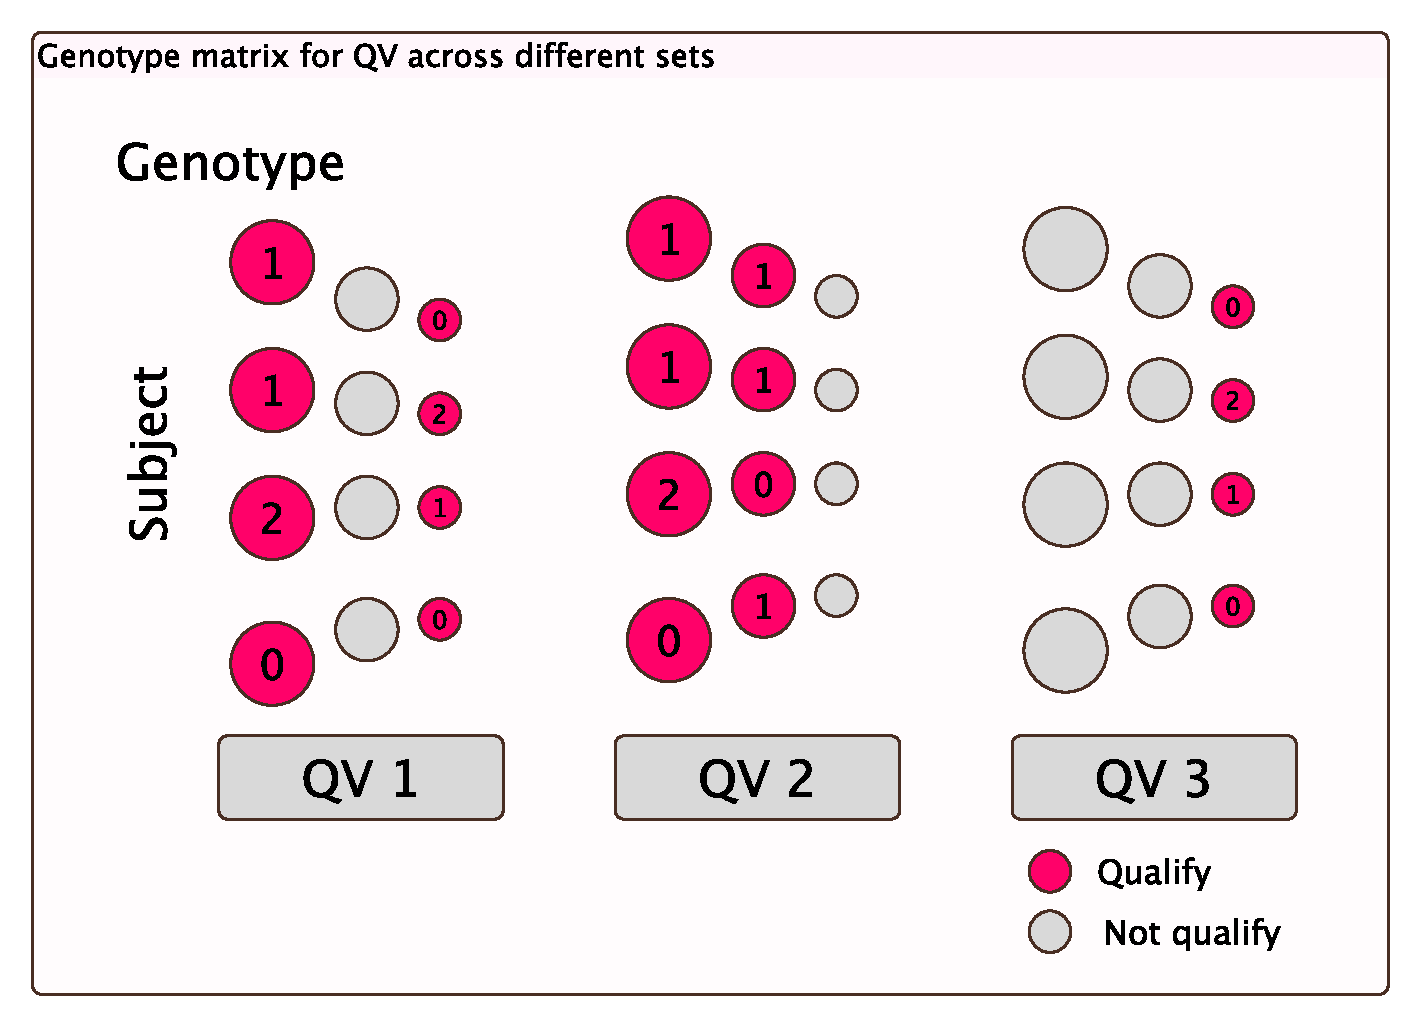
\includegraphics[width=0.99\textwidth]{./images/qv_matrix.pdf}
    \caption{Genotype matrices for three layers of \ac{qv} analysed in genetic studies. Each matrix represents a specific set, showing the genotypes of three individuals for three \ac{snp}s (\ac{snp}1, \ac{snp}2, \ac{snp}3). 
Genotypes of each \ac{snp} are coded as 0 (homozygous reference), 1 (heterozygous), and 2 (homozygous alternative).    
    In the \ac{qv}1 layer, \ac{snp}1 and \ac{snp}3 qualify as a \ac{qv} (highlighted in red). }
    \label{fig:qv_matrix}
\end{figure}

\subsubsection{Applications in complex data and multiblock fusion} 

Multiblock data fusion, an emerging field in statistics and machine learning championed by multi-omics, offers profound opportunities to unravel complex biological systems. By integrating multiple omics data types, DNA, RNA, protein, or clinical data, into a coherent analytical framework, researchers can uncover nuanced inter-dataset relationships that were previously obscured. Studies by \citet{kong2018nature} and \citet{howe2021within} have demonstrated that complex signals may reside within single datasets, underscoring the value of advanced fusion techniques. We contend that standardised and optimised \ac{qv} protocols not only advance omics research but also open up new theoretical domains. For instance, integrating various \ac{qv} sets on a single data source may facilitate joint analysis of associational, causal, and counterfactual relationships alongside traditional analyses, ultimately preparing a unified dataset for complex multi-omic investigations.

\subsubsection{Protocol development and standardisation needs} 
The complexity of multi-omic approaches necessitates clear protocols for merging data from different layers, ensuring that each component contributes meaningfully without conflating distinct signals. A standardised definition and reporting style for \ac{qv} are crucial for rapid theory development, particularly when data are not publicly available and codebases are complex and nuanced. Detailed, explicit protocols that list standardised definitions and variables, such as our demonstrated example for \ac{qv}1, will enhance reproducibility and foster new analytical frameworks.


\subsection{Future directions and implications} 
\subsubsection{Integration strategies}

New publishing formats like Registered Reports promote transparency and reproducibility \cite{chambers2014instead}, and a similar approach for \ac{qv} standardisation could expedite the clinical translation of genetic research. As machine learning and artificial intelligence models become increasingly capable of integrating vast multi-omic datasets, accurately formatted and curated \ac{qv}s will be essential. Particularly in rare diseases, where raw data may be insufficient for robust model training, refined \ac{qv} protocols can enrich feature representations, thereby improving predictive accuracy
\cite{barto2020looking}. 
The development of advanced \ac{qv} protocols is critical for statistical methods that navigate complex, interrelated omic data blocks \cite{smilde_multiblock_2022}. We advocate for a refined, comprehensive use of \ac{qv}s that goes beyond traditional single-stage filters to meet the sophisticated demands of modern multi-omic research.

\subsubsection{Notation typical to GWAS, VSAT, and other statistical applications}
We explore the notational use of \ac{qv} in commonly used applications to demonstrate how the conceptual framework can accelerate adoption in theoretical domains. 
For example, in GWAS \cite{uffelmann2021genome} the notation for the logistic regression model for estimating the probability of case status is given by:

$$
\text{logit}(p_i) = \log\left(\frac{p_i}{1 - p_i}\right) = \beta_0 + \sum_{k=1}^n \beta_k x_{ik} + \beta_{\text{geno}} G_i
$$
where \( p_i \) is the estimated probability that individual \( i \) is a case, \( \beta_0 \) is the intercept, \( \beta_k \) are coefficients for covariates \( x_{ik} \), and \( \beta_{\text{geno}} \) is the genetic effect coefficient for the genotype \( G_i \) (coded as 0, 1, or 2). An explicit version incorporating \ac{qv} notation is:
$$
\text{logit}(p_i) = \beta_0 + \beta_1\,\text{sex}_i + \beta_2\,\text{log10(age)}_i + \sum_{j=1}^{10} \beta_{2+j}\,\text{PC}_j^{(i)} + \sum_{k=1}^{n} \beta_{13+k}\,G_{\ac{qv}_{i,v,k}}
$$
where \( \beta_{13+k} \) represents the effect of each additional qualifying variant set \( k \) and \( G_{\ac{qv}_{i,v,k}} \) denotes the genotype for variant \( v \) in the \( k \)-th \ac{qv} set for individual \( i \).

Likewise, \ac{skat} and its optimal unified version, \ac{skat}-O, 
are used for association tests that accommodate multiple variants within a set (i.e. gene), accounting for their potentially differing directions and magnitudes of effects
\cite{wu2011rare, lee2012optimal}. 
The logistic regression model for \ac{skat}, taking into account the specific variants from the QV set, can be described as follows:
$$
\log \left( \frac{P}{1-P} \right) = X_i \gamma + G_{\text{QV}_{i,v}} \beta
$$
where:
\( P \) is the disease probability,
\( \gamma \) is an \( s \times 1 \) vector of regression coefficients of covariates,
\( \beta \) is an \( m \times 1 \) vector of regression coefficients for genetic variants,
\( G_{\text{QV}_{i,v}} \) denotes the genotype values for all variants \( v \) in the QV set for individual \( i \).
The \ac{skat} statistic is then:
$$
Q_S = (y - \hat{\pi})^\top K (y - \hat{\pi})
$$
where \( \hat{\pi} \) is the vector of the estimated probability of \( y \) under the null model, and \( K \) is the kernel matrix defined as \( G_{\text{QV}} W G_{\text{QV}}^\top \), with \( W \) being the diagonal weight matrix for the variants.

With these familiar examples established, we can consider more complex models where other variants outside of the main \ac{qv} set can be assessed,  $QV_{1,...,n} $,
which we describe in the next section. 
These sets can represent different categorisations or stratifications of genetic variants that might be relevant under varying analytical conditions or specific studies.

\subsubsection{Conceptual framework and statistical representation}

In \ac{gwas}, the transition from empirically testable variants (\ac{qv}1) to theoretical \ac{ax} marks a pivotal stage. The term \ac{ax} refers to genetic variants that ideally conform to fundamental genetic principles and are considered correct by genetic doctrine. However, due to technological constraints and gaps in understanding, \ac{ax} remains largely theoretical due to sequencing or detection difficulty. In contrast, \ac{qv}1 consists of variants from \ac{ax} that survive rigorous empirical filtering, applying standard \ac{gwas} pre-processing criteria (e.g. missing genotype data, \ac{maf}, Hardy-Weinberg equilibrium deviations, and individual missing data thresholds) to ensure data quality and relevance.

It is important to emphasise that we refer to unobserved or unknown variants, in the Bayesian sense, rather than \ac{vus}. The mathematical relationship between \ac{ax} and \ac{qv}1 can be expressed as follows:
\begin{align*}
\text{TP} &= \ac{qv}_{ax} \cap \ac{qv}1, \quad \text{(true positives)}\\[1ex]
\text{FN} &= \ac{qv}_{ax} \setminus \ac{qv}1, \quad \text{(false negatives)}\\[1ex]
\text{Unknowns} &= |\ac{qv}_{ax}| - |\text{TP}|,
\end{align*}
where TP represents the true positives that are both theoretically ideal and empirically robust, FN represents false negatives (theoretical variants erroneously excluded), and Unknowns quantifies the theoretical variants remaining untested. This structured approach clarifies the trade-offs in \ac{wgs} pre-processing by balancing data quality against the risk of overlooking significant genetic contributors.


In genomics, Bayesian statistics combines prior knowledge with empirical data to refine our understanding of the genetic variant landscape, particularly for variants beyond current empirical detection. We define a prior distribution \(P(\theta)\) based on established data (e.g. mutation rates and population variant frequencies) and combine it with the likelihood \(P(D\mid\theta)\) from the pre-processed genomic dataset (\ac{qv}1) using Bayes' theorem:
$$
P(\theta\mid D) = \frac{P(D\mid\theta) \, P(\theta)}{P(D)}.
$$
This posterior distribution updates our initial beliefs with the observed data. The ``unknowns'' - the theoretically possible variants not detected in \ac{qv}1 - are quantified as:
$$
\text{Unknowns} = \int_{\theta \in \Theta_{\text{unobserved}}} P(\theta\mid D) \, d\theta,
$$
where \(\Theta_{\text{unobserved}}\) represents the parameter space of undetected variants. 
By accounting for both the observed/unobserved known \ac{qv} and (estimating) theoretically possible but unknowable \ac{qv}, we can drastically increase our confidence scores.

This brief demonstration of potential future directions concludes our discussion of the methodological framework and its practical applications.

\section{Conclusions}
We emphasise the critical importance of \ac{qv} standardisation in genomics. By proposing a clear framework for integrating \ac{qv} protocols into analysis pipelines, we demonstrate that systematic handling of these variables enhances reproducibility, accuracy, and efficiency in genetic studies. As genomic technologies and data complexities continue to evolve, robust, scalable, and adaptable \ac{qv} protocols become ever more essential. Future work should extend these frameworks to accommodate emerging technologies and analytical challenges, thereby improving the fidelity and utility of genomic data interpretation across diverse applications.

\section{Funding}
This project was supported through the grant NDS-2021-911 (SwissPedHealth) from the Swiss Personalized Health Network and the Strategic Focal Area 'Personalized Health and Related Technologies' of the ETH Domain (Swiss Federal Institutes of Technology).

\section{Acknowledgements}
Acknowledgements We would like to thank all the patients and families who have been providing advice on SwissPedHealth and its projects, as well as the clinical and research teams at the participating institutions.

\section{Contributions}
DL designed the work and contributed to the manuscript.
AS, SB, VS, SÖ, JA contributed to the manuscript.
JF, JV, LJS supervised the work and applied for funding.

\section{Competing interests}
None declared.

\section{Collaborators}
The SwissPedHealth consortium may be named here for publication and is prepared as a comment in the LaTeX document.
% SwissPedHealth consortium: Andrea Agostini (Department of Computer Science, Institute for Machine Learning, ETH Zurich, Zurich, Switzerland), Anita Rauch (Institute of Medical Genetics, University of Zurich, Zurich, Switzerland), Anna Hartung (Inselspital, Bern University Hospital, University of Bern, Switzerland), Audrey van Drogen (PHRT Swiss Multi-Omics Centre [SMOC], ETH Zurich, Zurich, Switzerland \& Institute of Translational Medicine [ITM], Department of Health Sciences and Technology [D-HEST], ETH Zurich, Zurich, Switzerland), Aurélie Martin Necker (Patient and Family Advisory Committee, SwissPedHealth), Ben D Spycher (Institute of Social and Preventive Medicine [ISPM], University of Bern, Bern, Switzerland), Christian Kahlert (Ostschweizer Kinderspital, St Gallen, Switzerland), Christopher B Forrest (Center for Applied Clinical Research, Children’s Hospital of Philadelphia, Philadelphia, USA), Claudia E Kuehni (Institute of Social and Preventive Medicine [ISPM], University of Bern, Bern, Switzerland \& Division of Paediatric Respiratory Medicine and Allergology, Children's University Hospital, Inselspital, University of Bern, Bern, Switzerland), Cornelia Hagman (Department of Intensive Care and Neonatology and Children’s Research Centre, University Children’s Hospital Zurich, University of Zurich, Zurich, Switzerland), D Sean Froese (Division of Metabolism and Children’s Research Centre, University Children’s Hospital Zurich, University of Zurich, Zurich, Switzerland), Daphné Chopard (Department of Computer Science, Institute for Machine Learning, ETH Zurich, Zurich, Switzerland \& Department of Intensive Care and Neonatology and Children’s Research Centre, University Children’s Hospital Zurich, University of Zurich, Zurich, Switzerland), Dylan Lawless (School of Life Sciences, Ecole Polytechnique Fédérale de Lausanne, Lausanne, Switzerland \& Department of Intensive Care and Neonatology and Children’s Research Centre, University Children’s Hospital Zurich, University of Zurich, Zurich, Switzerland), Effy Vayena (Department of Health Sciences and Technology, Institute of Translational Medicine, ETH Zurich, Zurich, Switzerland), Eirini I Petrou (Department of Health Sciences and Technology, Institute of Translational Medicine, ETH Zurich, Zurich, Switzerland), Emanuele Palumbo (Department of Computer Science, Institute for Machine Learning, ETH Zurich, Zurich, Switzerland), Eric Giannoni (Clinic of Neonatology, Lausanne University Hospital, University of Lausanne, Lausanne, Switzerland), Fabiën N Belle (Institute of Social and Preventive Medicine [ISPM], University of Bern, Bern, Switzerland), Ioannis Xenarios (PHRT Swiss Multi-Omics Centre [SMOC], EPFL, Lausanne, Switzerland \& Department of Computational Biology, University of Lausanne, Lausanne, Switzerland \& Health 2030 Genome Center, Foundation Campus Biotech, Geneva, Switzerland), Jacques Fellay (School of Life Sciences, Ecole Polytechnique Fédérale de Lausanne, Lausanne, Switzerland \& Biomedical Data Science Center, Lausanne University Hospital, University of Lausanne, Lausanne, Switzerland), Jana Pachlopnik Schmid (Division of Immunology and Children’s Research Centre, University Children’s Hospital Zurich, University of Zurich, Zurich, Switzerland), Julia A Bielicki (Paediatric Research Center, University Children's Hospital Basel [UKBB], University of Basel, Basel, Switzerland \\& Centre for Neonatal and Paediatric Infection, St George’s, University of London, London, UK), Julia E Vogt (Department of Computer Science, Institute for Machine Learning, ETH Zurich, Zurich, Switzerland), Kathrin Hofmann (Patient and Family Advisory Committee, SwissPedHealth), Katrin Männik (PHRT Swiss Multi-Omics Centre [SMOC], EPFL, Lausanne, Switzerland \\& Center for Integrative Genomics, University of Lausanne, Lausanne, Switzerland \& Health 2030 Genome Center, Foundation Campus Biotech, Geneva, Switzerland), Keith Harshman (PHRT Swiss Multi-Omics Centre [SMOC], EPFL, Lausanne, Switzerland \& Health 2030 Genome Center, Foundation Campus Biotech, Geneva, Switzerland), Kelly Ormond (Department of Health Sciences and Technology, Institute of Translational Medicine, ETH Zurich, Zurich, Switzerland \& Department of Genetics, Stanford University School of Medicine, Stanford, California, USA), Klara Posfay-Barbe (Hôpitaux Universitaires de Genève, Geneva, Switzerland), Léa Ho Dac (Division of Paediatric Respiratory Medicine and Allergology, Department of Paediatrics, Inselspital, Bern University Hospital, University of Bern, Switzerland), Lorenz M Leuenberger (Institute of Social and Preventive Medicine [ISPM], University of Bern, Bern, Switzerland), Luregn J Schlapbach (Department of Intensive Care and Neonatology and Children’s Research Centre, University Children’s Hospital Zurich, University of Zurich, Zurich, Switzerland \& Child Health Research Centre, The University of Queensland, Brisbane, Australia), Manon Jaboyedoff (Pediatric Infectious Diseases and Vaccinology Unit, Service of Pediatrics, Department Mother-Woman-Child, Lausanne University Hospital and University of Lausanne, Lausanne, Switzerland), Mariam Ait Oumelloul (School of Life Sciences, Ecole Polytechnique Fédérale de Lausanne, Lausanne, Switzerland), Martin Stocker (Luzerner Kantonsspital, Luzern, Switzerland), Matthias R Baumgartner (Division of Metabolism and Children’s Research Centre, University Children’s Hospital Zurich, University of Zurich, Zurich, Switzerland), Nicola Zamboni (PHRT Swiss Multi-Omics Centre [SMOC], ETH Zurich, Zurich \& Institute of Molecular Systems Biology, ETH Zurich, Zurich, Switzerland), Nicole Goebel (Research and Analyses Services, Digitalisation \& ICT Division, University Hospital Basel, Basel, Switzerland), Patrick G A Pedrioli (PHRT Swiss Multi-Omics Centre [SMOC], ETH Zurich, Zurich, Switzerland \& Institute of Translational Medicine [ITM], Department of Health Sciences and Technology [D-HEST], ETH Zurich, Zurich, Switzerland \& Swiss Institute of Bioinformatics, Lausanne, Switzerland \& Department of Biology, Institute of Molecular Systems Biology, Swiss Federal Institute of Technology/ETH Zürich, Zurich, Switzerland), Philipp Latzin (Division of Paediatric Respiratory Medicine and Allergology, Department of Paediatrics, Inselspital, Bern University Hospital, University of Bern, Switzerland), Rebeca Mozun (Department of Intensive Care and Neonatology and Children’s Research Centre, University Children’s Hospital Zurich, University of Zurich, Zurich, Switzerland), Roger Lauener (Ostschweizer Kinderspital, St Gallen, Switzerland), Sandra Goetze (PHRT Swiss Multi-Omics Centre [SMOC], ETH Zurich, Zurich, Switzerland \& Institute of Translational Medicine [ITM], Department of Health Sciences and Technology [D-HEST], ETH Zurich, Zurich, Switzerland), Seraina Prader (Division of Immunology and Children’s Research Centre, University Children’s Hospital Zurich), Simon Boutry (School of Life Sciences, Ecole Polytechnique Fédérale de Lausanne, Lausanne, Switzerland), Sven Schulzke (Department of Neonatology, University Children's Hospital Basel [UKBB], University of Basel, Basel, Switzerland), Tatjana Welzel (Paediatric Research Center, University Children's Hospital Basel [UKBB], University of Basel, Basel, Switzerland), Thomas M Sutter (Department of Computer Science, Institute for Machine Learning, ETH Zurich, Zurich, Switzerland), Varvara Dimopoulou (Clinic of Neonatology, Lausanne University Hospital and University of Lausanne, Lausanne, Switzerland), Vito RT Zanotelli (Division of Metabolism and Children’s Research Centre, University Children’s Hospital Zurich, University of Zurich, Zurich, Switzerland), Xeni Deligianni (Research and Analyses Services, Digitalisation \& ICT Division, University Hospital Basel, Basel, Switzerland), Xenia Bovermann (Division of Paediatric Respiratory Medicine and Allergology, Department of Paediatrics, Inselspital, Bern University Hospital, University of Bern, Switzerland), Yara Shoman (Institute of Social and Preventive Medicine [ISPM], University of Bern, Bern, Switzerland).

\clearpage
\bibliographystyle{unsrtnat}
\bibliography{references} 

\end{document}
